\documentclass[]{book}
\usepackage{lmodern}
\usepackage{amssymb,amsmath}
\usepackage{ifxetex,ifluatex}
\usepackage{fixltx2e} % provides \textsubscript
\ifnum 0\ifxetex 1\fi\ifluatex 1\fi=0 % if pdftex
  \usepackage[T1]{fontenc}
  \usepackage[utf8]{inputenc}
\else % if luatex or xelatex
  \ifxetex
    \usepackage{mathspec}
  \else
    \usepackage{fontspec}
  \fi
  \defaultfontfeatures{Ligatures=TeX,Scale=MatchLowercase}
\fi
% use upquote if available, for straight quotes in verbatim environments
\IfFileExists{upquote.sty}{\usepackage{upquote}}{}
% use microtype if available
\IfFileExists{microtype.sty}{%
\usepackage[]{microtype}
\UseMicrotypeSet[protrusion]{basicmath} % disable protrusion for tt fonts
}{}
\PassOptionsToPackage{hyphens}{url} % url is loaded by hyperref
\usepackage[unicode=true]{hyperref}
\hypersetup{
            pdftitle={DAEs},
            pdfauthor={Jan Heiland},
            pdfborder={0 0 0},
            breaklinks=true}
\urlstyle{same}  % don't use monospace font for urls
\usepackage{natbib}
\bibliographystyle{apalike}
\usepackage{longtable,booktabs}
% Fix footnotes in tables (requires footnote package)
\IfFileExists{footnote.sty}{\usepackage{footnote}\makesavenoteenv{long table}}{}
\usepackage{graphicx,grffile}
\makeatletter
\def\maxwidth{\ifdim\Gin@nat@width>\linewidth\linewidth\else\Gin@nat@width\fi}
\def\maxheight{\ifdim\Gin@nat@height>\textheight\textheight\else\Gin@nat@height\fi}
\makeatother
% Scale images if necessary, so that they will not overflow the page
% margins by default, and it is still possible to overwrite the defaults
% using explicit options in \includegraphics[width, height, ...]{}
\setkeys{Gin}{width=\maxwidth,height=\maxheight,keepaspectratio}
\IfFileExists{parskip.sty}{%
\usepackage{parskip}
}{% else
\setlength{\parindent}{0pt}
\setlength{\parskip}{6pt plus 2pt minus 1pt}
}
\setlength{\emergencystretch}{3em}  % prevent overfull lines
\providecommand{\tightlist}{%
  \setlength{\itemsep}{0pt}\setlength{\parskip}{0pt}}
\setcounter{secnumdepth}{5}
% Redefines (sub)paragraphs to behave more like sections
\ifx\paragraph\undefined\else
\let\oldparagraph\paragraph
\renewcommand{\paragraph}[1]{\oldparagraph{#1}\mbox{}}
\fi
\ifx\subparagraph\undefined\else
\let\oldsubparagraph\subparagraph
\renewcommand{\subparagraph}[1]{\oldsubparagraph{#1}\mbox{}}
\fi

% set default figure placement to htbp
\makeatletter
\def\fps@figure{htbp}
\makeatother

\usepackage{booktabs}
\usepackage{booktabs}
\usepackage{longtable}
\usepackage{array}
\usepackage{multirow}
\usepackage{wrapfig}
\usepackage{float}
\usepackage{colortbl}
\usepackage{pdflscape}
\usepackage{tabu}
\usepackage{threeparttable}
\usepackage{threeparttablex}
\usepackage[normalem]{ulem}
\usepackage{makecell}
\usepackage{xcolor}

\title{DAEs}
\author{Jan Heiland}
\providecommand{\institute}[1]{}
\institute{OVGU/MPI}
\date{2020-05-01}

\usepackage{amsthm}
\newtheorem{theorem}{Theorem}[chapter]
\newtheorem{lemma}{Lemma}[chapter]
\newtheorem{corollary}{Corollary}[chapter]
\newtheorem{proposition}{Proposition}[chapter]
\newtheorem{conjecture}{Conjecture}[chapter]
\theoremstyle{definition}
\newtheorem{definition}{Definition}[chapter]
\theoremstyle{definition}
\newtheorem{example}{Example}[chapter]
\theoremstyle{definition}
\newtheorem{exercise}{Exercise}[chapter]
\theoremstyle{remark}
\newtheorem*{remark}{Remark}
\newtheorem*{solution}{Solution}
\let\BeginKnitrBlock\begin \let\EndKnitrBlock\end
\begin{document}
\maketitle

{
\setcounter{tocdepth}{1}
\tableofcontents
}
\chapter*{Preface}\label{preface}
\addcontentsline{toc}{chapter}{Preface}

This is a writeup of the introduction and, maybe, some other aspects of
my lectures on DAEs at the OVGU Magdeburg.

Fixes and feature requests can be submitted to the
\href{https://github.com/highlando/script-daes}{github-repo}.

\newcommand{\ind}{\operatorname{ind}}

\chapter{Introduction}\label{introduction}

Differential-algebraic equations (DAEs) are coupled differential- and
algebraic equations. DAEs often describe dynamical processes -- here are
the differential equations -- that are subject to constraints: the
algebraic equations.

Throughout this lecture, the free variable will be the time \(t\) and
differentiation will always be considered with respect to \(t\).

\section{Examples}\label{examples}

\textbf{Free fall vs.~the pendulum}

\begin{figure}

{\centering 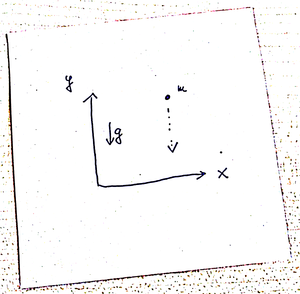
\includegraphics[width=0.4\linewidth]{pics/freefall} 

}

\caption{Free fall of a point mass.}\label{fig:free-fall}
\end{figure}

Free fall: Newton's second law applies:

\begin{quote}
\texttt{force\ =\ mass*acceleration}
\end{quote}

In 2D, the \(x\), \(y\) coordinates of a point of mass \(m\):

\begin{align*}
m\ddot x &= 0 \\
m\ddot y &= -mg
\end{align*}

where \(g\) is the gravity; see Figure \ref{fig:free-fall}.

Now \textbf{the pendulum}:

\emph{The same point mass attached to a string}.

\begin{figure}

{\centering 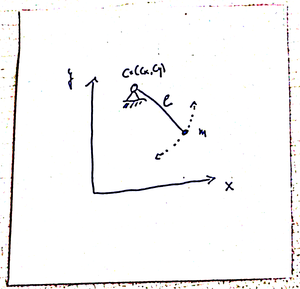
\includegraphics[width=0.4\linewidth]{pics/pendulum} 

}

\caption{A pendulum.}\label{fig:pendulum}
\end{figure}

Again, we have \texttt{force\ =\ mass*acceleration} but also the
conditions that the mass moves on a circle:

\[
 (x(t) - c_x)^2 + (y(t) - c_y)^2 = l^2,
\] where \((c_x, c_y)\) are the coordinates of the center and \(l\) is
the length of the string; see Figure \ref{fig:pendulum}.

We use the Langrangian function to derive the equations of motion. For
the pendulum, we have the kinetic energy \(T\), the potential \(U\), and
the constraint \(h\) as

\[
  T = \frac 12 m (\dot x(t)^2 + \dot y(t)^2), \quad U = mgy, \quad \text{and} \quad h = (x(t) - c_x)^2 + (y(t) - c_y)^2 - l^2 .
\]

Thus, from the principle that

\[
\frac{d}{dt}(\frac{\partial L}{\partial \dot q}) - \frac{\partial L}{\partial q} = 0, \quad\text{for}\quad L = U -T - \lambda h \quad\text{and}\quad q=x, y ,\lambda
\]

one obtains:

\begin{longtable}[]{@{}lr@{}}
\toprule
generalized coordinate & equation\tabularnewline
\midrule
\endhead
\(q \leftarrow x\) &
\(m\ddot x(t) + 2 \lambda(t) (x(t) - c_x) = 0\)\tabularnewline
\(q \leftarrow y\) &
\(m\ddot y(t) + mgy + 2 \lambda(t) (y(t) - c_y) = 0\)\tabularnewline
\(q \leftarrow \lambda\) &
\((x(t) - c_x)^2 + (y(t) - c_y)^2 - l^2 =0\)\tabularnewline
\bottomrule
\end{longtable}

\BeginKnitrBlock{example}[The Pendulum]
\protect\hypertarget{exm:the-pendulum}{}{\label{exm:the-pendulum}
\iffalse (The Pendulum) \fi{} } After an order reduction via the new
variables \(u:=\dot x\) and \(v=\dot y\) the overall system reads

\begin{equation}
\begin{split}
\dot x &= u \\
\dot y &= v \\
\dot u &= - 2 \lambda (x - c_x) \\ 
\dot v &= - 2 \lambda (y - c_y) - mgy \\
0&=(x - c_x)^2 + (y - c_y)^2 - l^2, 
\end{split}
\label{eq:pendulum}
\end{equation}

where we have omitted the time dependence.
\EndKnitrBlock{example}

Equation \eqref{eq:pendulum} is a canonical example for a DAE with
combined differential and algebraic equations.

\textbf{Electrical Circuits}

Another class of DAEs arises from the modelling electrical circuits. We
consider the example of \emph{charging a conductor through a resistor}
as illustrated in Figure \ref{fig:circuit}.

\begin{figure}

{\centering 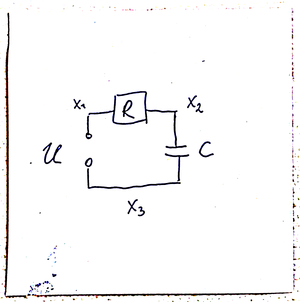
\includegraphics[width=0.4\linewidth]{pics/circuit} 

}

\caption{Electrical circuit with a source, a resistor, and a conductor.}\label{fig:circuit}
\end{figure}

We formulate the problem in terms of the potentials \(x_1\), \(x_2\),
\(x_3\), that are assumed to reside in the wires between a source \(U\)
and a resistor \(R\), the resistor \(R\) and the capacitor \(C\), and
the capacitor and the source.

A model for the circuit is given through the following principles and
considerations.

\begin{itemize}
\tightlist
\item
  the source defines the difference in the neighboring potentials:
  \(x_1 - x_3 - U = 0\)
\item
  the current \(I_R\) that is induced by the potentials neighboring the
  resistor is is defined through \emph{Ohm's law}:
  \(I_R = \frac{x_1 - x_2}{R}\)
\item
  the current \(I_C\) that is induced by the potentials neighboring the
  capacitor is described through: \(I_C = C(\dot x_3 - \dot x_2)\)
\item
  \emph{Kirchhoff's law} states that everywhere in the circuit the
  currents sum up to zero:
  \(I_C + I_R = C(\dot x_3 - \dot x_2)+ \frac{x_1 - x_2}{R}=0\)
\item
  finally, we can set a ground potential (note that so far all equations
  only consider differences in the potential) and we set \(x_3 = 0\).
\end{itemize}

\BeginKnitrBlock{example}
\protect\hypertarget{exm:the-circuit}{}{\label{exm:the-circuit} }Summing all
up, the equations that model the circuit are given as

\begin{equation}
\begin{split}
C(\dot x_3 - \dot x_2) &= - \frac{x_1 - x_2}{R} \\
0  &= x_1 - x_3 - U \\
0 &= x_3. 
\end{split}
\label{eq:circuit}
\end{equation}
\EndKnitrBlock{example}

\textbf{Navier-Stokes Equations}

The Navier-Stokes equations (NSE) are commonly used to model all kind of
flows. They describe the evolution of the velocity \(v\) of the fluid
and the pressure \(p\) in the fluid. Note that the flow occupies a
spatial domain, say in \(\mathbb R^{3}\) so that \(v\) and \(p\) are
functions both of the time variable \(t\) and a space variable \(\xi\):

\[
v\colon (t, \xi) \mapsto v(t,\xi)\in \mathbb R^{3} \quad\text{and}\quad  p\colon (t, \xi) \mapsto p(t,\xi)\in \mathbb R.
\]

The NSE:

\begin{align*}
  \frac{\partial v}{\partial t} + (v\otimes \nabla_\xi)v - \Delta_\xi v + \nabla_\xi p &= 0, \\
  \nabla_\xi \cdot v &= 0,
\end{align*}

with \(\otimes\) denoting the outer product and \(\nabla_\xi\) and
\(\Delta_\xi\) denoting the gradient and the \emph{Laplace} operator. If
we only count the derivatives with respect to time, as postulated in the
introduction, the NSE can be seen as an (abstract) DAE.

\textbf{Automatic Modelling or \emph{Engineers vs.~Mathematicians}}

If a system, say an engine, consists of many interacting processes, it
is convenient and common practice to model the dynamics of each
particular process and to couple the subprocesses through interface
conditions.

This coupling is done through equating quantities so that the overall
model will consist of dynamical equations of the subprocesses and
algebraic relations at the interfaces -- which makes it a DAE.

In fact, tools like \href{https://www.modelica.org/}{\texttt{modelica}}
for automatic modelling of complex processes do exactly this.

The approach of \emph{automatic modelling} is universal and convenient
for engineers. However, the resulting model equations will be DAEs
which, as we will see, pose particular problems in their analytical and
numerical treatment.

\section{Why are DAEs difficult to
treat}\label{why-are-daes-difficult-to-treat}

Firstly, DAEs do not have the smoothing properties of ODEs, where the
solution is one degree smoother than the right hand side. Secondly, the
algebraic constraints are essential for the validity of the model. Thus,
a numerical approximation may render the model infeasible.

\textbf{Non-smooth Solutions}

\BeginKnitrBlock{example}
\protect\hypertarget{exm:nonsmooth-sols}{}{\label{exm:nonsmooth-sols}
}Consider the equation

\begin{align*}
    \dot x_1(t) &= x_2(t) \\
        0 & = x_2(t) -g(t)
\end{align*}

where \(g\) can be a nonsmooth function like

\[
    g(t) = 
    \begin{cases} 
        0, \quad\text{if}\quad t < 1 \\
        1, \quad\text{if}\quad t \geq 1 \\
    \end{cases}
\]

In this case the solution part \(x_1=const. + \int_0^tg(s)ds\) will be a
smooth function and the solution part \(x_2=g\) will have jumps.
\EndKnitrBlock{example}

Even worse

\begin{quote}
\emph{the solution of a DAE may depend on derivatives of the right hand
sides.}
\end{quote}

This observation indicates that certain difficulties will arise since

\begin{itemize}
\tightlist
\item
  numerical approximation schemes require smoothness of the solutions
\item
  differentiation is numerically ill-posed unlike numerical integration
\end{itemize}

\textbf{Numerical Solution Means Approximation}

Imagine the equations \eqref{eq:pendulum} that describe the pendulum are
solved approximately. Then, the algebraic constraint will be violated,
i.e.~the point mass will leave the circle and the obtained numerical
solution becomes infeasible.

Thus, special care has to be taken of the algebraic constraints when the
equations of motions are numerically integrated.

\chapter{Basic Definitions and
Notions}\label{basic-definitions-and-notions}

We consider DAEs in the general form

\begin{equation}
    F(t, x, \dot x) = 0
    \label{eq:gendae}
\end{equation}

with \(F\colon I \times D_x \times D_{\dot x} \to \mathbb R^m\) and with
a time interval \(I=[t_0,t_e] \subset \mathbb R\) and state spaces
\(D_x\), \(D_{\dot x} \subset \mathbb R^{n}\) and the task to find a
function

\begin{equation*}
    x \colon I \to \mathbb R^{n}
\end{equation*}

with time derivative \(\dot x \colon I \to \mathbb R^{n}\) such that
\eqref{eq:gendae} is fulfilled for all \(t\in I\).

A dynamical process that evolves in time needs an initial state. Thus,
one can expect a unique solution to the DAEs only if an initial value is
prescribed

\begin{equation}
    x(t_0) = x_0 \in \mathbb R^{n}. \label{eq:gendaeiniv} 
\end{equation}

\section{Solution Concept}\label{solution-concept}

In order to talk of solutions, we need to define what we understand as a
solution.

\BeginKnitrBlock{definition}
\protect\hypertarget{def:dae-solution}{}{\label{def:dae-solution} } 1. A
function \(x \in \mathcal C^1(I, \mathbb R^{n})\) is called a
\emph{solution to the DAE} \eqref{eq:gendae}, if
\(F(t, x(t), \dot x(t)) = 0\) holds for all \(t\in I\).

\begin{enumerate}
\def\labelenumi{\arabic{enumi}.}
\setcounter{enumi}{1}
\item
  A function \(x \in \mathcal C^1(I, \mathbb R^{n})\) is called a
  \emph{solution to the initial value problem} \eqref{eq:gendae} and
  \eqref{eq:gendaeiniv}, if, furthermore, \(x(t_0)= x_0\) holds.
\item
  An initial condition \eqref{eq:gendaeiniv} is called consistent for the
  DAE \eqref{eq:gendae}, if there exists at least one solution as defined
  in 2.
\end{enumerate}
\EndKnitrBlock{definition}

Some remarks

\begin{itemize}
\tightlist
\item
  The requirement that \(x \in \mathcal C^1\) could be relaxed. Compare
  Example \ref{exm:nonsmooth-sols}, where certain components of the
  solution where smoother than others.
\item
  Consistency of initial values is a major issue in the treatment of
  DAEs. See the pendulum\ldots{}
\end{itemize}

\section{Initial Conditions and
Consistency}\label{initial-conditions-and-consistency}

We consider again the equations of motions of the pendulum (Example
\ref{exm:the-pendulum})

\begin{align*}
    \dot x(t) &= u(t) \\
    \dot y(t) &= v(t) \\
    \dot u(t) &= - 2 \lambda(t) (x(t) - c_x) \\ 
    \dot v(t) &= - 2 \lambda(t) (y(t) - c_y) - mgy
\end{align*}

with the constraint

\begin{equation}
    0=(x(t) - c_x)^2 + (y(t) - c_y)^2 - l^2. \label{eq:pendulum-rvst-cnstrt}
\end{equation}

To use this model to predict the time evolution of the system, a
starting point needs to be known, say for \(t=0\). This means initial
positions and initial velocities:

\[
\begin{bmatrix} 
x(0) \\ y(0)
\end{bmatrix}
=
\begin{bmatrix} 
    x_0 \\ y_0
\end{bmatrix}
\quad\text{and}\quad
\begin{bmatrix} 
u(0) \\ v(0)
\end{bmatrix}
=
\begin{bmatrix} 
    u_0 \\ v_0.
\end{bmatrix}
\]

The constraint \eqref{eq:pendulum-rvst-cnstrt} needs to be fulfilled at
all times and also at \(t=0\), which gives the constraint for the
initial positions:

\begin{equation*}
    (x_0 - c_x)^2 + (y_0 - c_y)^2 - l^2=0.
\end{equation*}

Moreover, if a constraint \(g(x(t), y(t))=0\) holds for all \(t\), then,
necessarily, \(\frac{d}{dt}g=0\) for all \(t\). For the pendulum this
means that

\begin{equation}
    2(x(t) - c_x)u(t) + 2(y(t) - c_y)v(t) = 0 \label{eq:pendulum-rvst-cnstrt-ddt}
\end{equation}

must hold for all \(t\) and in particular at \(t=0\) which gives
constraints on the initial velocities \(u_0\) and \(v_0\):

\begin{equation*}
    2(x_0 - c_x)u_0 + 2(y_0 - c_y)v_0 = 0.
\end{equation*}

Some remarks on consistency, constraints, and derivations:

\begin{itemize}
\tightlist
\item
  The so-called \emph{consistency conditions} on
  \((x_0, y_0, u_0, v_0)\) have the physical interpretation that the
  initial positions lie on the prescribed circle and that the velocities
  are tangent to this circle.
\item
  One can show that the variable \(\lambda\) is completely defined in
  terms of \(x\) and \(y\) and their derivatives. Thus, in the
  formulation \eqref{eq:pendulum}, both in the analysis and in the
  numerical treatment, there is no need for an initial value for
  \(\lambda\). However, as we will see, DAEs can be reformulated as ODEs
  through differentiation and substitutions. In such an ODE formulation,
  a necessary initial condition for \(\lambda\) will have to fulfill
  similar consistency conditions as \((x_0, y_0, u_0, v_0)\).
\end{itemize}

Condition \eqref{eq:pendulum-rvst-cnstrt-ddt} is an example for a
\emph{hidden-constraint} -- an algebraic constraint to the system that
is not explicit in the original formulation. In theory, condition
\eqref{eq:pendulum-rvst-cnstrt} can be replaced by
\eqref{eq:pendulum-rvst-cnstrt-ddt}. Moreover, through differentiation and
elimination of constraints, a DAE can be brought into the form of an
ODE: in the case of the circuit of Example \ref{exm:the-circuit} one
only needs to replace the constraints by their derivatives:

\begin{equation}
\begin{split}
C(\dot x_3 - \dot x_2) &= - \frac{x_1 - x_2}{R} \\
\dot x_1 - \dot x_3 &= \dot U \\
\dot x_3 &= 0. 
\end{split}
\label{eq:circuit-ddt}
\end{equation}

Note that \eqref{eq:circuit-ddt} can be written as \(B\dot x = Ax + f\)
with an invertible matrix \(B\) and, thus, is an ODE.

For an ODE there is no constraint on the initial values. However, a
solution to \eqref{eq:circuit-ddt} only solves the original DAE
\eqref{eq:circuit}, if the initial values are consistent with the DAE. In
this case, this means \(x_3(t_0)=0\) and
\(x_1(t_0) - x_3(t_0) = U(t_0)\).

\chapter{Linear DAEs with Constant
Coefficients}\label{linear-daes-with-constant-coefficients}

\BeginKnitrBlock{definition}
\protect\hypertarget{def:drazin-inverse}{}{\label{def:drazin-inverse} } Let
\(E\in \mathbb C^{n,n}\) and \(\nu = \ind(E)\). A matrix
\(X\in \mathbb C^{n,n}\) that fulfills

\begin{align}
    EX & = XE, \label{eq:def-drazin-a} \\
    XEX & = X, \label{eq:def-drazin-b} \\
    XE^{\nu+1} & = E^{\nu}, \label{eq:def-drazin-c}
\end{align}

is called a \emph{Drazin inverse} of \(E\).
\EndKnitrBlock{definition}

With the following theorem we confirm that a Drazin inverse to a matrix
\(E\) is unique so that we can write \(E^D\) for it.

\BeginKnitrBlock{theorem}
\protect\hypertarget{thm:drazin-inverse-unique}{}{\label{thm:drazin-inverse-unique}
} Every matrix \(E\in\mathbb{C}^{n,n}\) has one, and only one, Drazin
inverse.
\EndKnitrBlock{theorem}

\BeginKnitrBlock{proof}
\iffalse{} {Proof. } \fi{}Uniqueness: Let \(X_1\) and \(X_2\) be two
Drazin inverses of \(E\). Then by repeated application of the identities
in \eqref{eq:def-drazin-a}--\eqref{eq:def-drazin-c} one derives that

\begin{align*}
X_1 EX_1 E X_2 =   &X_1EX_2 = X_1EX_2EX_2  \\
X_1^2 E^2 X_2 = \dotsm=   &X_1EX_2 = \dotsm= X_1E^2X_2^2  \\
X_1^{\nu+1}E^{\nu+1} X_2 =\dotsm=\dotsm=   &X_1EX_2 =\dotsm=\dotsm= X_1E^{\nu+1}X_2^{\nu+1}  \\
X_1^{\nu+1}E^{\nu+1} X_1 =\dotsm=\dotsm=\dotsm=   &X_1EX_2 =\dotsm=\dotsm=\dotsm= X_2E^{\nu+1}X_2^{\nu+1}  \\
X_1 =\dotsm=\dotsm=\dotsm=\dotsm=   &X_1EX_2 =\dotsm=\dotsm=\dotsm=\dotsm= X_2, \\
\end{align*}

where in the second last step we used the identities

\[
    E^{\nu+1}X_1=X_1E^{\nu+1}=E^{\nu}=X_2E^{\nu+1}=E^{\nu+1}X_2.
\]
\EndKnitrBlock{proof}

\newcommand{\rank}{\operatorname{rank}}
\newcommand{\kernel}{\operatorname{kernel}}
\newcommand{\corange}{\operatorname{corange}}
\newcommand{\range}{\operatorname{range}}
\newcommand{\cokernel}{\operatorname{cokernel}}

\chapter{Linear DAEs with Time-varying
Coefficients}\label{linear-daes-with-time-varying-coefficients}

\BeginKnitrBlock{theorem}
\protect\hypertarget{thm:local-canonical-form}{}{\label{thm:local-canonical-form}
}Let \(E, A \in \mathbb C^{m,n}\) and let

\begin{equation}
T,~Z,~T',~V \label{eq:lcf-subspaces}
\end{equation}

be

\begin{longtable}[]{@{}ll@{}}
\toprule
Matrix & as the basis of\tabularnewline
\midrule
\endhead
\(T\) & \(\kernel E\)\tabularnewline
\(Z\) & \(\corange E = \kernel E^H\)\tabularnewline
\(T'\) & \(\cokernel E = \range E^H\)\tabularnewline
\(V\) & \(\corange (Z^HAT)\)\tabularnewline
\bottomrule
\end{longtable}

then the quantities

\begin{equation}
r,~a,~s,~d,~u,~v \label{eq:lcf-quantities}
\end{equation}

defined as

\begin{longtable}[]{@{}lll@{}}
\toprule
Quantity & Definition & Name\tabularnewline
\midrule
\endhead
\(r\) & \(\rank E\) & \emph{rank}\tabularnewline
\(a\) & \(\rank (Z^HAT)\) & \emph{algebraic part}\tabularnewline
\(s\) & \(\rank (V^HZ^HAT')\) & \emph{strangeness}\tabularnewline
\(d\) & \(r-s\) & \emph{differential part}\tabularnewline
\(u\) & \(n-r-a\) & \emph{undetermined variables}\tabularnewline
\(v\) & \(m-r-a-s\) & \emph{vanishing equations}\tabularnewline
\bottomrule
\end{longtable}

are invariant under local equivalence transformations and \((E, A)\) is
locally equivalent to the canonical form

\begin{equation}
\left(\begin{bmatrix}
I_s & 0 & 0 & 0 \\
0 & I_d & 0 & 0 \\
0 & 0 & 0 & 0 \\
0 & 0 & 0 & 0 \\
0 & 0 & 0 & 0
\end{bmatrix},
\begin{bmatrix}
0 & 0 & 0 & 0  \\
0 & 0 & 0 & 0  \\
0 & 0 & I_a & 0 \\
I_s & 0 & 0 & 0 \\
0 & 0 & 0 & 0
\end{bmatrix}\right),
\label{eq:local-canonical-form}
\end{equation}

where all diagonal blocks are square, except maybe the last one.
\EndKnitrBlock{theorem} Some remarks on the spaces and how the names are
derived for the case \(E\dot x = Ax +f\) with constant coefficients. The
ideas are readily transferred to the case with time-varying
coefficients.

Let \[x(t) = Ty(t) + T'y'(t),\]

where \(y\) denotes the components of \(x\) that evolve in the range of
\(T\) and \(y'\) the respective complement. (Since \([T|T']\) is a basis
of \(\mathbb C^{n}\), there exist such \(y\) and \(y'\) that uniquely
define \(x\) and vice versa). With \(T\) spanning \(\ker E\) we find
that

\[E \dot x(t) = ET\dot y(t) + ET'\dot y'(t)\]

so that the DAE basically reads

\[ET'\dot y'(t) = ATy(t) + AT'y'(t)+f,\]

i.e.~the components of \(x\) defined through \(y\) are, effectively, not
differentiated. With \(Z\) containing exactly those \(v\), for which
\(v^HE=0\), it follows that

\[Z^HET'\dot y'(t) = 0 = Z^HATy(t) + Z^HAT'y'(t)+Z^Hf,\]

or

\[Z^HATy(t) = -Z^HAT'y'(t)-Z^Hf,\]

so that \(\rank Z^HAT\) indeed describes the number of purely algebraic
equations and variables in the sense that it defines parts of \(y\)
(which is never going to be differentiated) in terms of algebraic
relations (no time derivatives are involved).

With the same arguments and with \(V=\corange Z^HAT\), it follows that

\[V^HZ^HAT'y'(t) = -V^HZ^HATy(t) -V^HZ^Hf=-V^HZ^Hf,\]

is the part of \(E\dot x = Ax + f\) in which those components \(y'\)
that are also differentiated are algebraically equated to a right-hand
side. This is the \emph{strangeness} (rather in the sense of
\emph{skewness}) of DAEs that variables can be both differential and
algebraic. Accordingly, \(\rank V^HZ^HAT'\) describes the size of the
skewness component.

\begin{quote}
\textbf{Outlook}: If there is no strangeness, the DAE is called
strangeness-free. Strangeness can be eliminated through iterated
differentiation and substitution. The needed number of such iterations
(that is independent of the the size \(s\) of the \emph{strange} block
here) will define the strangeness index.
\end{quote}

\BeginKnitrBlock{example}
\protect\hypertarget{exm:strangeness-in-the-circuit}{}{\label{exm:strangeness-in-the-circuit}
}With basic scalings and state transforms, one finds for the
coefficients of Example \ref{exm:the-circuit} that: \[
(E, A) \backsim 
\left(
\begin{bmatrix} I_2 & 0 \\ 0 & 0 \end{bmatrix}
,
\begin{bmatrix} 0 & 0 \\ 0 & I_1 \end{bmatrix}
\right).
\]

We compute the subspaces as defined in \eqref{eq:lcf-subspaces}:

\begin{longtable}[]{@{}ll@{}}
\toprule
\begin{minipage}[b]{0.16\columnwidth}\raggedright\strut
Matrix\strut
\end{minipage} & \begin{minipage}[b]{0.34\columnwidth}\raggedright\strut
as the basis of/computed as\strut
\end{minipage}\tabularnewline
\midrule
\endhead
\begin{minipage}[t]{0.16\columnwidth}\raggedright\strut
\(T=\begin{bmatrix} 0 \\ I_1 \end{bmatrix}\)\strut
\end{minipage} & \begin{minipage}[t]{0.34\columnwidth}\raggedright\strut
\(\kernel\begin{bmatrix} I_2 & 0 \\ 0 & 0 \end{bmatrix}\)\strut
\end{minipage}\tabularnewline
\begin{minipage}[t]{0.16\columnwidth}\raggedright\strut
\(Z=\begin{bmatrix} 0 \\ I_1 \end{bmatrix}\)\strut
\end{minipage} & \begin{minipage}[t]{0.34\columnwidth}\raggedright\strut
\(\corange\begin{bmatrix} I_2 & 0 \\ 0 & 0 \end{bmatrix}=\kernel\begin{bmatrix} I_2 & 0 \\ 0 & 0 \end{bmatrix}^H\)\strut
\end{minipage}\tabularnewline
\begin{minipage}[t]{0.16\columnwidth}\raggedright\strut
\(T'=\begin{bmatrix} I_2 \\ 0 \end{bmatrix}\)\strut
\end{minipage} & \begin{minipage}[t]{0.34\columnwidth}\raggedright\strut
\(\cokernel\begin{bmatrix} I_2 & 0 \\ 0 & 0 \end{bmatrix}=\range\begin{bmatrix} I_2 & 0 \\ 0 & 0 \end{bmatrix}^H\)\strut
\end{minipage}\tabularnewline
\begin{minipage}[t]{0.16\columnwidth}\raggedright\strut
\(Z^HAT=I_1\)\strut
\end{minipage} & \begin{minipage}[t]{0.34\columnwidth}\raggedright\strut
\(\begin{bmatrix} 0 \\ I_1 \end{bmatrix}^H\begin{bmatrix} 0 & 0 \\ 0 & I_1 \end{bmatrix}\begin{bmatrix} 0 \\ I_1 \end{bmatrix}\)\strut
\end{minipage}\tabularnewline
\begin{minipage}[t]{0.16\columnwidth}\raggedright\strut
\(V=0\)\strut
\end{minipage} & \begin{minipage}[t]{0.34\columnwidth}\raggedright\strut
\(\corange (Z^HAT) = \kernel I_1^H\phantom{\begin{bmatrix} 0 \\ I_1 \end{bmatrix}}\)\strut
\end{minipage}\tabularnewline
\begin{minipage}[t]{0.16\columnwidth}\raggedright\strut
\(Z^HAT'=0_{2\times 1}\)\strut
\end{minipage} & \begin{minipage}[t]{0.34\columnwidth}\raggedright\strut
\(\begin{bmatrix} 0 \\ I_1 \end{bmatrix}^H\begin{bmatrix} 0 & 0 \\ 0 & I_1 \end{bmatrix}\begin{bmatrix} I_2 \\ 0 \end{bmatrix}\)\strut
\end{minipage}\tabularnewline
\bottomrule
\end{longtable}

and derive the quantities as defined in \eqref{eq:lcf-quantities}:

\begin{longtable}[]{@{}lll@{}}
\toprule
Name & Value & Derived from\tabularnewline
\midrule
\endhead
rank & \(r=2\) &
\(\rank E = \rank \begin{bmatrix} I_2 & 0 \\ 0 & 0 \end{bmatrix}\)\tabularnewline
algebraic part & \(a=1\) & \(\rank Z^HAT = \rank I_1\)\tabularnewline
strangeness & \(s=0\) &
\(\rank V^HZ^HAT' = \rank 0_{2\times 1}\)\tabularnewline
differential part & \(d=2\) & \(d=r-s=2-0\)\tabularnewline
undetermined variables & \(u=0\) & \(u=n-r-a=3-2-1\)\tabularnewline
vanishing equations & \(v=0\) & \(v=m-r-a-s=3-2-1-0\)\tabularnewline
\bottomrule
\end{longtable}
\EndKnitrBlock{example}

\BeginKnitrBlock{example}
\protect\hypertarget{exm:strangeness-in-the-nse}{}{\label{exm:strangeness-in-the-nse}
}With more involved scalings and state transforms, one finds for the
coefficients of the linearized and spatially discretized Navier-Stokes
equations (see Exercise I) that: \[
(\mathcal E, \mathcal A) =
\left(
\begin{bmatrix} M & 0 \\ 0 & 0 \end{bmatrix}
,
\begin{bmatrix} A & B^H \\ B & 0 \end{bmatrix}
\right)
\backsim 
\left(
\begin{bmatrix} I_{n_1} & 0 & 0 \\ 0 & I_{n_2} & 0 \\ 0 & 0 & 0\end{bmatrix}
,
\begin{bmatrix} A_{11} & A_{12} & I_{n_1} \\ A_{21} & A_{22} & 0 \\ I_{n_1} & 0 & 0\end{bmatrix}
\right).
\]

We compute the subspaces as defined in \eqref{eq:lcf-subspaces}:

\begin{longtable}[]{@{}ll@{}}
\toprule
\begin{minipage}[b]{0.17\columnwidth}\raggedright\strut
Matrix\strut
\end{minipage} & \begin{minipage}[b]{0.37\columnwidth}\raggedright\strut
as the basis of/computed as\strut
\end{minipage}\tabularnewline
\midrule
\endhead
\begin{minipage}[t]{0.17\columnwidth}\raggedright\strut
\(T=\begin{bmatrix} 0 \\ 0 \\I_{n_1} \end{bmatrix}\)\strut
\end{minipage} & \begin{minipage}[t]{0.37\columnwidth}\raggedright\strut
\(\kernel \begin{bmatrix} I_{n_1} & 0 & 0 \\ 0 & I_{n_2} & 0 \\ 0 & 0 & 0\end{bmatrix}\)\strut
\end{minipage}\tabularnewline
\begin{minipage}[t]{0.17\columnwidth}\raggedright\strut
\(Z=\begin{bmatrix} 0 \\ 0 \\I_{n_1} \end{bmatrix}\)\strut
\end{minipage} & \begin{minipage}[t]{0.37\columnwidth}\raggedright\strut
\(\corange \begin{bmatrix} I_{n_1} & 0 & 0 \\ 0 & I_{n_2} & 0 \\ 0 & 0 & 0\end{bmatrix}\)\strut
\end{minipage}\tabularnewline
\begin{minipage}[t]{0.17\columnwidth}\raggedright\strut
\(T'=\begin{bmatrix} I_{n_1} & 0 \\ 0 & I_{n_2} \\ 0 & 0 \end{bmatrix}\)\strut
\end{minipage} & \begin{minipage}[t]{0.37\columnwidth}\raggedright\strut
\(\cokernel\begin{bmatrix} I_{n_1} & 0 & 0 \\ 0 & I_{n_2} & 0 \\ 0 & 0 & 0\end{bmatrix}\)\strut
\end{minipage}\tabularnewline
\begin{minipage}[t]{0.17\columnwidth}\raggedright\strut
\(Z^HAT=0_{n_1}\)\strut
\end{minipage} & \begin{minipage}[t]{0.37\columnwidth}\raggedright\strut
\(\begin{bmatrix} 0 \\ 0 \\I_{n_1} \end{bmatrix}^H\begin{bmatrix} A_{11} & A_{12} & I_{n_1} \\ A_{21} & A_{22} & 0 \\ I_{n_1} & 0 & 0\end{bmatrix}\begin{bmatrix} 0 \\ 0 \\I_{n_1} \end{bmatrix}\)\strut
\end{minipage}\tabularnewline
\begin{minipage}[t]{0.17\columnwidth}\raggedright\strut
\(V=I_{n_1}\)\strut
\end{minipage} & \begin{minipage}[t]{0.37\columnwidth}\raggedright\strut
\(\corange (Z^HAT) = \kernel 0_{n_1}^H\phantom{\begin{bmatrix} 0 \\ I_1 \end{bmatrix}}\)\strut
\end{minipage}\tabularnewline
\begin{minipage}[t]{0.17\columnwidth}\raggedright\strut
\(Z^HAT'=\begin{bmatrix} I_{n_1} & 0_{n_1\times n_2}\end{bmatrix}\)\strut
\end{minipage} & \begin{minipage}[t]{0.37\columnwidth}\raggedright\strut
\(\begin{bmatrix} 0 \\ 0 \\I_{n_1} \end{bmatrix}^H\begin{bmatrix} A_{11} & A_{12} & I_{n_1} \\ A_{21} & A_{22} & 0 \\ I_{n_1} & 0 & 0\end{bmatrix}\begin{bmatrix} I_{n_1} & 0 \\ 0 & I_{n_2} \\ 0 & 0 \end{bmatrix}\)\strut
\end{minipage}\tabularnewline
\bottomrule
\end{longtable}

and derive the quantities as defined in \eqref{eq:lcf-quantities}:

\begin{longtable}[]{@{}lll@{}}
\toprule
\begin{minipage}[b]{0.24\columnwidth}\raggedright\strut
Name\strut
\end{minipage} & \begin{minipage}[b]{0.10\columnwidth}\raggedright\strut
Value\strut
\end{minipage} & \begin{minipage}[b]{0.37\columnwidth}\raggedright\strut
Derived from\strut
\end{minipage}\tabularnewline
\midrule
\endhead
\begin{minipage}[t]{0.24\columnwidth}\raggedright\strut
rank\strut
\end{minipage} & \begin{minipage}[t]{0.10\columnwidth}\raggedright\strut
\(r=n_1+n_2\)\strut
\end{minipage} & \begin{minipage}[t]{0.37\columnwidth}\raggedright\strut
\(\rank E = \rank \begin{bmatrix} I_{n_1} & 0 & 0 \\ 0 & I_{n_2} & 0 \\ 0 & 0 & 0\end{bmatrix}\)\strut
\end{minipage}\tabularnewline
\begin{minipage}[t]{0.24\columnwidth}\raggedright\strut
algebraic part\strut
\end{minipage} & \begin{minipage}[t]{0.10\columnwidth}\raggedright\strut
\(a=0\)\strut
\end{minipage} & \begin{minipage}[t]{0.37\columnwidth}\raggedright\strut
\(\rank Z^HAT = \rank 0_{n_1}\)\strut
\end{minipage}\tabularnewline
\begin{minipage}[t]{0.24\columnwidth}\raggedright\strut
strangeness\strut
\end{minipage} & \begin{minipage}[t]{0.10\columnwidth}\raggedright\strut
\(s=n_1\)\strut
\end{minipage} & \begin{minipage}[t]{0.37\columnwidth}\raggedright\strut
\(\rank V^HZ^HAT' = \rank \begin{bmatrix} I_{n_1} & 0_{n_1\times n_2}\end{bmatrix}\)\strut
\end{minipage}\tabularnewline
\begin{minipage}[t]{0.24\columnwidth}\raggedright\strut
differential part\strut
\end{minipage} & \begin{minipage}[t]{0.10\columnwidth}\raggedright\strut
\(d=n_2\)\strut
\end{minipage} & \begin{minipage}[t]{0.37\columnwidth}\raggedright\strut
\(d=r-s=(n_1 + n_2) - n_1\)\strut
\end{minipage}\tabularnewline
\begin{minipage}[t]{0.24\columnwidth}\raggedright\strut
undetermined variables\strut
\end{minipage} & \begin{minipage}[t]{0.10\columnwidth}\raggedright\strut
\(u=n_1\)\strut
\end{minipage} & \begin{minipage}[t]{0.37\columnwidth}\raggedright\strut
\(u=n-r-a=(n_1+n_2+n_1)-(n_1+n_2)-0\)\strut
\end{minipage}\tabularnewline
\begin{minipage}[t]{0.24\columnwidth}\raggedright\strut
vanishing equations\strut
\end{minipage} & \begin{minipage}[t]{0.10\columnwidth}\raggedright\strut
\(v=0\)\strut
\end{minipage} & \begin{minipage}[t]{0.37\columnwidth}\raggedright\strut
\(v=m-r-a-s=(n_1+n_2+n_1)-(n_1+n_2)-n_1\)\strut
\end{minipage}\tabularnewline
\bottomrule
\end{longtable}
\EndKnitrBlock{example}

\BeginKnitrBlock{theorem}[see Kunkel/Mehrmann, Thm. 3.9]
\protect\hypertarget{thm:continuous-svd}{}{\label{thm:continuous-svd}
\iffalse (see Kunkel/Mehrmann, Thm. 3.9) \fi{} } Let
\(E\in \mathcal C^l(I, \mathbb C^{m,n})\) with \(\rank E(t)=r\) for all
\(t\in I\). Then there exist smooth and pointwise unitary (and, thus,
nonsingular) matrix functions \(U\) and \(V\), such that

\[
 U^HEV =
 \begin{bmatrix}
 \Sigma & 0 \\
 0 & 0
 \end{bmatrix}
\] with pointwise nonsingular
\(\Sigma \in \mathcal C^l(I, \mathbb C^{r,r})\).
\EndKnitrBlock{theorem}

\BeginKnitrBlock{theorem}
\protect\hypertarget{thm:global-canonical-form}{}{\label{thm:global-canonical-form}
} Let \(E, A \in \mathcal C^l(I, \mathbb C^{m,n})\) be sufficiently
smooth and suppose that

\begin{equation}
    r(t) = r, \quad a(t)=a, \quad s(t)=s \label{eq:glob-local-char-vals}
\end{equation}

for the local characteristic values of \((E(t), A(t))\). Then \((E, A)\)
is globally equivalent to the canonical form

\begin{equation}
\left(
\begin{bmatrix}
I_s &  0  & 0 & 0 \\
0   & I_d & 0 & 0 \\
0   &  0  & 0 & 0 \\
0   &  0  & 0 & 0 \\
0   &  0  & 0 & 0
\end{bmatrix}, 
\begin{bmatrix}
0   & A_{12}&  0  & A_{14} \\
0   &   0   &  0  & A_{24} \\
0   &   0   & I_a & 0 \\
I_s &   0   &  0  & 0 \\
0   &   0   &  0  & 0
\end{bmatrix}
\right ).
\label{eq:glob-can-form}
\end{equation}

All entries are again matrix functions on \(I\) and the last block
column in both matrix functions of \eqref{eq:glob-can-form} has size
\(u=n-s-d-a\).
\EndKnitrBlock{theorem}

\BeginKnitrBlock{proof}
\iffalse{} {Proof. } \fi{}In what follows, we will tacitly redefine the
block matrix entries that appear after the global equivalence
transformations. The first step is the continous SVD of \(E\); see
Theorem \ref{thm:global-canonical-form}.

\begin{align*}
(E,A) & 
\sim   
\left(\begin{bmatrix}
\Sigma & 0 \\
0 & 0
\end{bmatrix},
\begin{bmatrix}
A_{11} & A_{12} \\
A_{21} & A_{22}
\end{bmatrix}\right) \\
%%%%%%%%%%%%%%%%%%%%%%%%%%
& \sim   
\left(\begin{bmatrix}
I_r & 0 \\
0 & 0
\end{bmatrix},
\begin{bmatrix}
A_{11} & A_{12} \\
A_{21} & A_{22}
\end{bmatrix}\right) \\
%%%%%%%%%%%%%%%%%%%%%%
& \sim   
\left(\begin{bmatrix}
I_r & 0 \\
0 & 0
\end{bmatrix},
\begin{bmatrix}
A_{11} & A_{12}V_1 \\
U_1^HA_{21} & U_1^HA_{22}V_1 
\end{bmatrix}
-
\begin{bmatrix} I_r & 0 \\ 0 & 0 \end{bmatrix}
\begin{bmatrix} 0 & 0 \\ 0 & \dot V_1 \end{bmatrix}
\right) \\
%%%%%%%%%%%%%%%%%%%%%%
& \sim   
\left(\begin{bmatrix}
I_r & 0 & 0 \\
0 & 0 & 0 \\
0 & 0 & 0
\end{bmatrix},
\begin{bmatrix}
A_{11} & A_{12} & A_{13}\\
A_{21} & I_a & 0 \\
A_{31} & 0  & 0
\end{bmatrix}\right) \\
%%%%%%%%%%%%%%%%%%%%%%
& \sim   
\left(\begin{bmatrix}
V_2 & 0 & 0 \\
0 & 0 & 0 \\
0 & 0 & 0
\end{bmatrix},
\begin{bmatrix}
A_{11}V_2 & A_{12} & A_{13}\\
A_{21}V_2 & I_a & 0 \\
U_2^HA_{31}V_2 & 0 & 0
\end{bmatrix}
-
\begin{bmatrix}
\dot I_r & 0 & 0 \\
0 & 0 & 0 \\
0 & 0 & 0
\end{bmatrix}
\begin{bmatrix}
\dot V_2 & 0 & 0 \\
0 & 0 & 0 \\
0 & 0 & 0
\end{bmatrix} \right)\\
%%%%%%%%%%%%%%%%%%%%%%
& \sim   
\left(\begin{bmatrix}
V_{11} & V_{12} & 0 & 0 \\
V_{21} & V_{22} & 0 & 0 \\
0 & 0 & 0 & 0 \\
0 & 0 & 0 & 0 \\
0 & 0 & 0 & 0
\end{bmatrix},
\begin{bmatrix}
A_{11} & A_{12} & A_{13} & A_{14}  \\
A_{21} & A_{22} & A_{23} & A_{24}  \\
A_{31} & A_{32} & I_a & 0 \\
I_s & 0 & 0 & 0 \\
0 & 0 & 0 & 0
\end{bmatrix} \right)\\
%%%%%%%%%%%%%%%%%%%%%%
& \sim   
\left(\begin{bmatrix}
I_s & 0 & 0 & 0 \\
0 & I_d & 0 & 0 \\
0 & 0 & 0 & 0 \\
0 & 0 & 0 & 0 \\
0 & 0 & 0 & 0
\end{bmatrix},
\begin{bmatrix}
0 & A_{12} & A_{13} & A_{14}  \\
0 & A_{22} & A_{23} & A_{24}  \\
0 & A_{32} & I_a & 0 \\
I_s & 0 & 0 & 0 \\
0 & 0 & 0 & 0
\end{bmatrix} 
\begin{bmatrix}
I_s & 0 & 0 & 0  \\
0 & I_d & 0 & 0  \\
0 & -A_{32} & I_a & 0 \\
I_s & 0 & 0 & I_a
\end{bmatrix} 
\right) \\
%%%%%%%%%%%%%%%%%
& \sim   
\left(\begin{bmatrix}
I_s & 0 & 0 & 0 \\
0 & I_d & 0 & 0 \\
0 & 0 & 0 & 0 \\
0 & 0 & 0 & 0 \\
0 & 0 & 0 & 0
\end{bmatrix},
\begin{bmatrix}
0 & A_{12} & A_{13} & A_{14}  \\
0 & A_{22} & A_{23} & A_{24}  \\
0 & 0 & I_a & 0 \\
I_s & 0 & 0 & 0 \\
0 & 0 & 0 & 0
\end{bmatrix}\right)\\
%%%%%%%%%%%%%%%%%
& \sim   
\left(\begin{bmatrix}
I_s & 0 & 0 & 0 \\
0 & I_d & 0 & 0 \\
0 & 0 & 0 & 0 \\
0 & 0 & 0 & 0 \\
0 & 0 & 0 & 0
\end{bmatrix},
\begin{bmatrix}
0 & A_{12} & 0 & A_{14}  \\
0 & A_{22} & 0 & A_{24}  \\
0 & 0 & I_a & 0 \\
I_s & 0 & 0 & 0 \\
0 & 0 & 0 & 0
\end{bmatrix}\right)\\
%%%%%%%%%%%%%%%%%
& \sim   
\left(\begin{bmatrix}
I_s & 0 & 0 & 0 \\
0 & Q_2 & 0 & 0 \\
0 & 0 & 0 & 0 \\
0 & 0 & 0 & 0 \\
0 & 0 & 0 & 0
\end{bmatrix},
\begin{bmatrix}
0 & A_{12}Q_2 & 0 & A_{14}  \\
0 & A_{22}Q_2-\dot Q_2 & 0 & A_{24}  \\
0 & 0 & I_a & 0 \\
I_s & 0 & 0 & 0 \\
0 & 0 & 0 & 0
\end{bmatrix}\right) \\
%%%%%%%%%%%%%%%%%
& \sim   
\left(\begin{bmatrix}
I_s & 0 & 0 & 0 \\
0 & I_d & 0 & 0 \\
0 & 0 & 0 & 0 \\
0 & 0 & 0 & 0 \\
0 & 0 & 0 & 0
\end{bmatrix},
\begin{bmatrix}
0 & A_{12} & 0 & A_{14}  \\
0 & 0 & 0 & A_{24}  \\
0 & 0 & I_a & 0 \\
I_s & 0 & 0 & 0 \\
0 & 0 & 0 & 0
\end{bmatrix}\right),
\end{align*}

where the final equivalence holds, if \(Q_2\) is chosen as the (unique
and pointwise invertible) solution of the linear matrix valued ODE \[
\dot Q_2 = A_{22}(t)Q_2 ,  \quad Q_2 (t_0 ) = I_d.
\] Then, \(A_{22}\) vanishes because of the special choice of \(Q_2\)
and \(E_{22}\) becomes \(I_d\) after scaling the second block line by
\(Q_2^{-1}\).
\EndKnitrBlock{proof}

\chapter{Numerical Approximation of
DAEs}\label{numerical-approximation-of-daes}

In order to analyse the approximation error of the RKM
\((\mathcal A, \beta, \gamma)\) applied to a regular linear DAE with
constant coefficients

\[
 E\dot x = Ax+f(t).
\]

Without loss of generality, we can assume that

\begin{itemize}
\tightlist
\item
  \((E,A)\) is in Kronecker Canonical Form \(\leftarrow\) RKM are
  invariant under equivalence transformation
\item
  \((E,A)=(N,I)\) \(\leftarrow\) the \emph{regular part} can be treated
  by ODE theory
\item
  \(E=N=N_\nu\) consists of a single Jordan block \(\leftarrow\)
  otherwise consider each Jordan block separately
\end{itemize}

Thus, we can consider the special DAE

\begin{equation}
\begin{bmatrix}
0 & 1 &        &         &    \\
  & 0 & 1      &         &    \\
  &   & \ddots & \ddots  &    \\
  &   &        & 0       & 1  \\
  &   &        &         & 0 
\end{bmatrix}
\dot x = x + f(t),
\label{eq:spec-dae-rkm-cc}
\end{equation}

where

\[
 x(t) = \begin{bmatrix} x_1(t) \\ x_2(t) \\ \vdots \\ x_\nu(t) \end{bmatrix}
 \quad\text{and}\quad
 f(t) = \begin{bmatrix} f_1(t) \\ f_2(t) \\ \vdots \\ f_\nu(t) \end{bmatrix}
 \]

\BeginKnitrBlock{theorem}
\protect\hypertarget{thm:local-consistency-error-rkm-lcc}{}{\label{thm:local-consistency-error-rkm-lcc}
}The local error of an RKM with \(\mathcal A\) invertible applied to
\eqref{eq:spec-dae-rkm-cc} behaves like

\[
x(t_{i+1}) - x_{i+1} = \mathcal O(h^{\kappa_\nu - \nu + 2} + h^{\kappa_{\nu-1} - \nu + 3} + \cdots + h^{\kappa_1 +1})
\]

where \(\kappa_j\) is the maximum number such that

\begin{longtable}[]{@{}lll@{}}
\toprule
\begin{minipage}[b]{0.06\columnwidth}\raggedright\strut
\strut
\end{minipage} & \begin{minipage}[b]{0.38\columnwidth}\raggedright\strut
Condition\strut
\end{minipage} & \begin{minipage}[b]{0.23\columnwidth}\raggedright\strut
range of \(k\)\strut
\end{minipage}\tabularnewline
\midrule
\endhead
\begin{minipage}[t]{0.06\columnwidth}\raggedright\strut
a.)\strut
\end{minipage} & \begin{minipage}[t]{0.38\columnwidth}\raggedright\strut
\(\beta^T\mathcal A^{-k}e = \beta^T\mathcal A^{-j}\gamma^{j-k} / (j-k)!\)\strut
\end{minipage} & \begin{minipage}[t]{0.23\columnwidth}\raggedright\strut
\(k=1,2,\cdots,j-1\)\strut
\end{minipage}\tabularnewline
\begin{minipage}[t]{0.06\columnwidth}\raggedright\strut
b.)\strut
\end{minipage} & \begin{minipage}[t]{0.38\columnwidth}\raggedright\strut
\(\beta^T\mathcal A^{-j}\gamma^k = k! / (k-j+1)!\)\strut
\end{minipage} & \begin{minipage}[t]{0.23\columnwidth}\raggedright\strut
\(k=j,j+1,\cdots\)\strut
\end{minipage}\tabularnewline
\bottomrule
\end{longtable}

for all \(k\leq \kappa_j\) and for \(j=1, \cdots, \nu\).
\EndKnitrBlock{theorem}

\BeginKnitrBlock{proof}
\iffalse{} {Proof. } \fi{}Since we consider the pure consistency error,
we can assume that \(x_i=x(t_i)\). With that and with the definition of
the RKM, the error is given as \[
\tau = x(t_{i+1}) - x_{i+1} = -h\sum_{j=1}^s \beta_j \dot X_{ij} + \sum_{k\geq 1} \frac{h^k}{k!}x^{(k)}(t_i).
\]

Because of the special structure of the DAE, we can concentrate on the
first error component \(\tau_1\) \(\leftarrow\) the error component
\(\tau_2\) is the \emph{first} component of the problem of index
\(\nu-1\). For \(\tau_1\) we have the formula

\[
\tau_1 = x_1(t_{i+1}) - x_{i+1,1} = h\beta^T\sum_{j=1}^\nu (h\mathcal A)^{-j}Z_{ij} + \sum_{k\geq 1} \frac{h^k}{k!}x_1^{(k)}(t_i).
\]

One may confirm directly, or by means of the solution formula for
\(N\dot x = x + f\), that the \(\ell\)-th component of \(x\) is defined
as \[
x_\ell(t) = - \sum_{j=\ell}^{\nu}f_j^{(j-\ell)}(t).
\]

The componentwise Taylor expansion of \(Z_{i,\ell}\) reads

\begin{align*}
Z_{i\ell} 
&= 
\begin{bmatrix}
x_{i,\ell} + f_\ell(t_i+\gamma_1 h) \\
x_{i,\ell} + f_\ell(t_i+\gamma_2 h) \\
\vdots \\
x_{i,\ell} + f_\ell(t_i+\gamma_s h) 
\end{bmatrix}
=
\begin{bmatrix}
    x_{i,\ell} + f_\ell(t_i) + \sum_{k\geq 1}\frac{h^k}{k!}f_\ell^{(k)}(t_i)\gamma_1^k \\
  x_{i,\ell} + f_\ell(t_i) + \sum_{k\geq 1}\frac{h^k}{k!}f_\ell^{(k)}(t_i)\gamma_2 ^k \\
\vdots \\
  x_{i,\ell} + f_\ell(t_i) + \sum_{k\geq 1}\frac{h^k}{k!}f_\ell^{(k)}(t_i)\gamma_s ^k 
\end{bmatrix} \\
&=
x_{i,\ell}e+\sum_{k\geq 0} \frac{h^k}{k!}f_\ell^{(k)}(t_i)\gamma^k
\end{align*}

With that and with \(x_i=x(t_i)\), we expand the error \(\tau_1\) as
follows:

\begin{align*}
\tau_1 &= \beta^T\sum_{j=1}^\nu (h\mathcal A)^{-j}Z_{ij} + \sum_{k\geq 1} \frac{h^k}{k!}x_1^{(k)}(t_i)\\
&= \beta^T\sum_{j=1}^\nu h^{-j+1}\mathcal A^{-j}\bigr[ x_{j}(t_i)e+\sum_{k\geq 0} \frac{h^k}{k!}f_j^{(k)}(t_i)\gamma^k\bigr] \\&\quad\quad\quad\quad+ \sum_{k\geq 1} \frac{h^k}{k!}x_1^{(k)}(t_i)\\
&= \beta^T\sum_{j=1}^\nu h^{-j+1}\mathcal A^{-j}\bigr[ -\sum_{k=j}^{\nu}f_k^{(k-j)}(t_i)e+\sum_{k\geq 0} \frac{h^k}{k!}f_j^{(k)}(t_i)\gamma^k\bigr] \\&\quad\quad\quad\quad- \sum_{k\geq 1} \frac{h^k}{k!} \sum_{j=1}^{\nu}f_j^{(j-1+k)}(t_i)\\
&= -\sum_{j=1}^\nu \sum_{k=j}^{\nu} h^{-j+1}\beta^T\mathcal A^{-j} ef_k^{(k-j)}(t_i)+\sum_{j=1}^\nu \sum_{k\geq 0}\frac{h^{k-j+1}}{k!}\beta^T\mathcal A^{-j} \gamma^k f_j^{(k)}(t_i) \\&\quad\quad\quad\quad- \sum_{k\geq 1}\sum_{j=1}^{\nu} \frac{h^k}{k!} f_j^{(j-1+k)}(t_i),
\end{align*}

which, with
\(\sum_{j=1}^\nu \sum_{k=j}^\nu g(j,k) = \sum_{k=1}^\nu \sum_{j=1}^k g(j,k)= \sum_{k=1}^\nu \sum_{j=1}^k g(k,j)\),
becomes

\begin{align*}
\tau_1 &= \sum_{j=1}^{\nu} \bigl[ -\sum_{k=1}^j h^{-k+1}\beta^T\mathcal A^{-k} ef_k^{(j-k)}(t_i)\\&\quad\quad\quad\quad+\sum_{k\geq 0}\frac{h^{k-j+1}}{k!}\beta^T\mathcal A^{-j} \gamma^k f_j^{(k)}(t_i) \\&\quad\quad\quad\quad- \sum_{k\geq 1}\frac{h^k}{k!} f_j^{(j-1+k)}(t_i) \bigr] \\
 &= \sum_{j=1}^{\nu} \bigl[ -\sum_{k=1}^j h^{-k+1}\beta^T\mathcal A^{-k} ef_k^{(j-k)}(t_i)\\
 &\quad\quad\quad\quad+\sum_{k=0}^{j-1}\frac{h^{k-j+1}}{k!}\beta^T\mathcal A^{-j} \gamma^k f_j^{(k)}(t_i)+\sum_{k\geq j}\frac{h^{k-j+1}}{k!}\beta^T\mathcal A^{-j} \gamma^k f_j^{(k)}(t_i) \\&\quad\quad\quad\quad- \sum_{k\geq 1}\frac{h^k}{k!} f_j^{(j-1+k)}(t_i) \bigr].
\end{align*}

A shift of indices, \(\sum_{k=0}^{j-1}g(k)=\sum_{k=1}^j g(j-k)\) and
\(\sum_{k\geq 1}g(k)=\sum_{k\geq j}g(k-j+1)\), then gives:

\begin{align*}
    \tau_1 &= \sum_{j=1}^{\nu} \bigl[ -\sum_{k=1}^j h^{-k+1}\beta^T\mathcal A^{-k} ef_k^{(j-k)}(t_i)+\sum_{k=1}^{j}\frac{h^{-k+1}}{(j-k)!}\beta^T\mathcal A^{-j} \gamma^{j-k} f_j^{(j-k)}(t_i)\\ &\quad\quad\quad\quad+\sum_{k\geq j}\frac{h^{k-j+1}}{k!}\beta^T\mathcal A^{-j} \gamma^k f_j^{(k)}(t_i) - \sum_{k\geq j}\frac{h^{k-j+1}}{(k-j+1)!} f_j^{(k)}(t_i) \bigr].
\end{align*}
\EndKnitrBlock{proof}

\chapter{Construction and Analysis of RKM for nonlinear
DAEs}\label{construction-and-analysis-of-rkm-for-nonlinear-daes}

Now we consider RKM for nonlinear DAEs. We start with a DAE in
\emph{semi explicit} strangeness-free form and give general results on
how to write down a general RKM for it and how to analyse the global
error. Then, we consider general strangeness-free nonlinear DAEs and
show that a certain class of RKM applies well -- namely those that can
be constructed by collocation with Lagrange polynomials over the
\emph{Radau}, \emph{Lobatto}, or \emph{Gauss} quadrature points.

\section{General RKM for Semi-Explicit Strangeness-free
DAEs}\label{general-rkm-for-semi-explicit-strangeness-free-daes}

A semi explicit strangeness-free DAE is of the form

\begin{align}
\dot x &= f(t, x, y) \label{eq:semexp-dae-diff} \\
0 &= g(t, x, y) \label{eq:semexp-dae-alg}
\end{align}

with the Jacobian of \(g\) with respect to \(y\), i.e. \[
\partial_y\otimes g(t, x(t), y(t)) =: g_y(t, x(t), y(t)),
\] being invertible for all \(t\) along the solution \((x,y)\).

Some observations:

\begin{itemize}
\tightlist
\item
  this system is strangeness-free
\item
  under certain assumptions, any DAE can be brought into this form
\item
  in the linear case \(E\dot z = Az +f\), with \(z=(x,y)\), the
  assumptions basically mean that \[
   E = \begin{bmatrix} I & 0 \\ 0 & 0 \end{bmatrix} \quad\text{and}\quad 
   A = \begin{bmatrix} * & * \\ * & A_{22} \end{bmatrix},
  \] with \(A_{22}(t)\) invertible for all \(t\).
\item
  The condition \(g_y\) invertible means that, locally, one could
  consider \[
   \dot x = f(t, x, R(t,x)), \quad\text{with $R$ such that}\quad y=R(t,x).
  \] However, this is not practical for numerical purposes.
\end{itemize}

The general strategy to get a suitable formulation of a time
discretization of system
\eqref{eq:semexp-dae-diff}-\eqref{eq:semexp-dae-alg} by any RKM is to
consider the perturbed version

\begin{align*}
\dot x = f(t, x, y),  \\
\varepsilon \dot y = g(t, x, y),
\end{align*}

which is an ODE, formulate the RKM, and then let \(\varepsilon \to 0\).
In the Hairer/Wanner Book, this approach is called
*\(\varepsilon\)-embedding.

This is, consider

\begin{longtable}[]{@{}lll@{}}
\caption{\label{tab:RKM-semiexp-DAE} RKM applied to semi-explicit
DAEs}\tabularnewline
\toprule
\begin{minipage}[t]{0.25\columnwidth}\raggedright\strut
\(x_{i+1} = x_i + h\sum_{j=1}^s\beta_j \dot X_{ij}\),\strut
\end{minipage} & \begin{minipage}[t]{0.25\columnwidth}\raggedright\strut
\(y_{i+1} = y_i + h\sum_{j=1}^s\beta_j \dot Y_{ij}\),\strut
\end{minipage} & \begin{minipage}[t]{0.23\columnwidth}\raggedright\strut
\strut
\end{minipage}\tabularnewline
\begin{minipage}[t]{0.25\columnwidth}\raggedright\strut
\(\dot X_{ij} = f(t_i+\gamma_jh, X_{ij}, Y_{ij})\),\strut
\end{minipage} & \begin{minipage}[t]{0.25\columnwidth}\raggedright\strut
\(\varepsilon \dot Y_{ij} = g(t_i+\gamma_j h, X_{ij}, Y_{ij})\),\strut
\end{minipage} & \begin{minipage}[t]{0.23\columnwidth}\raggedright\strut
\(j=1,2,\cdots,s, \quad \quad (*)\)\strut
\end{minipage}\tabularnewline
\begin{minipage}[t]{0.25\columnwidth}\raggedright\strut
\(X_{ij} = x_i + h\sum_{\ell=1}^s\alpha_{j\ell}\dot X_{i\ell}\),\strut
\end{minipage} & \begin{minipage}[t]{0.25\columnwidth}\raggedright\strut
\(\phantom{\varepsilon}Y_{ij} = y_i + h\sum_{\ell=1}^s\alpha_{j\ell}\dot Y_{i\ell}\),\strut
\end{minipage} & \begin{minipage}[t]{0.23\columnwidth}\raggedright\strut
\(j=1,2,\cdots,s,\)\strut
\end{minipage}\tabularnewline
\bottomrule
\end{longtable}

i.e., the RKM applied to an ODE in the variables \((x,y)\), and replace
\((*)\) by

\[
\dot X_{ij} = f(t_i+\gamma_jh, X_{ij}, Y_{ij}),\quad 0 = g(t_i+\gamma_j h, X_{ij}, Y_{ij}), \quad j=1,2,\cdots,s.
\]

\BeginKnitrBlock{theorem}[Kunkel/Mehrmann Thm. 5.16]
\protect\hypertarget{thm:unnamed-chunk-1}{}{\label{thm:unnamed-chunk-1}
\iffalse (Kunkel/Mehrmann Thm. 5.16) \fi{} }Consider a semi-explicit,
strangeness-free DAE as in
\eqref{eq:semexp-dae-diff}-\eqref{eq:semexp-dae-alg} with a consistent
initial value \((x_0, y_0)\). The time-discretization by a RKM,

\begin{itemize}
\tightlist
\item
  with \(\mathcal A\) invertible and
  \(\rho:=1-\beta^T\mathcal A^{-1}e\),
\item
  applied as in Table \ref{tab:RKM-semiexp-DAE} with \(\varepsilon=0\),
\item
  that is convergent of order \(p\) for ODEs
\item
  and fulfills the \emph{Butcher condition} \(C(q)\) with \(q\geq p+1\)
\end{itemize}

leads to an global error that behaves like \[
\|\mathfrak X(t_N) - \mathfrak X_N\| = \mathcal O(h^k),
\]

where

\begin{itemize}
\tightlist
\item
  \(k=p\), if \(\rho=0\),
\item
  \(k=\min\{p, q+1\}\), if \(-1\leq \rho < 1\)
\item
  \(k=\min\{p, q-1\}\), if \(\rho =1\).
\end{itemize}

If \(|\rho|>1\), then the RKM -- applied to
\eqref{eq:semexp-dae-diff}--\eqref{eq:semexp-dae-alg} -- does not converge.
\EndKnitrBlock{theorem}

Some words on the conditions on \(p\), \(q\), and \(\rho\):

\begin{itemize}
\item
  For \emph{stiffly accurate} methods, \(\beta^T \mathcal A^{-1}e=1\)
  and, thus, \(\rho=0\) \(\rightarrow\) no order reduction for
  \emph{strangeness free} or \emph{index-1} systems
\item
  For the \emph{implicit midpoint rule} also known as the \emph{1-stage
  Gauss method}: \[
  \begin{array}{c|c}
  \frac 12 & \frac 12 \\
  \hline
   & 1  
  \end{array}
     \]

  \begin{itemize}
  \tightlist
  \item
    the convergence order for ODEs is \(p=2\)
  \item
    but
    \(1-\beta^T \mathcal A^{-1}e = 1- 1\cdot {\bigl(\frac 12\bigr)}^{-1} 1 = -1\),
    so that \(\min\{p-1, q\} = k \leq 1\), depending on \(q\).
  \item
    in fact \(k=1\) as \[
      C(q): \quad \sum_{\ell=1}^s\alpha_{j\ell}\gamma_\ell^{\bar k-1}=\frac{1}{\bar k} \gamma_j^{\bar k}, \quad {\bar k}=1,\cdots,q, \quad j=1,\cdots,s
      \] in the present case of \(s=1\),
    \(\alpha_{11}=\gamma_1=\frac 12\) is fulfilled for
    \({\bar k}=1: \quad \frac 12 = \frac 12\)
  \item
    it is not relevant here, but for
    \({\bar k}=2:\quad \frac 12 \cdot \frac 12 \neq \frac 12 \cdot \frac 14\)
  \end{itemize}
\end{itemize}

\section{Collocation RKM for Implicit Strangeness-free
DAEs}\label{collocation-rkm-for-implicit-strangeness-free-daes}

The general form of a \emph{strangeness-free} DAE is given as

\begin{align}
\hat F_1(t,x,\dot x) &= 0 \label{eq:impl-sf-dae-fone}\\
\hat F_2(t,x) &= 0 \label{eq:impl-sf-dae-ftwo}
\end{align}

where the \emph{strangeness-free} or \emph{index-1} assumption is
encoded in the existence of \emph{implicit functions} \(\mathcal L\),
\(\mathcal R\) such that, with \(x=(x_1,x_2)\), the implicit DAE
\eqref{eq:impl-sf-dae-fone}--\eqref{eq:impl-sf-dae-ftwo} is equivalent to
the semi-explicit DAE

\begin{align*}
  \dot x_1  &= \mathcal L(t,x_1,x_2) \\
   0 &= \mathcal R(t,x_1) -x_2
\end{align*}

In what follows we show that a \emph{collocation} approach coincides
with certain RKM discretizations so that the convergence analysis of the
RKM can be done via approximation theory.

\begin{quote}
Regression (Collocation): -- If one looks for a function
\(x\colon [0,1] \to \mathbb R^{}\) that fulfills \(F(x(t))=0\) for all
\(t\in[0,1]\), one may interpolate \(x\) by, say, a polynomial
\(x_p(t) = \sum_{\ell=0}^kx_\ell t^\ell\) and determine the \(k+1\)
coefficients \(x_\ell\) via the solution of the system of (nonlinear)
equations \(F(x_p(t_\ell))=0\), \(\ell=0,1,\dotsc,k\), where the
\(t_\ell\in[0,1]\) are the \(k+1\) \emph{collocation points}.
\end{quote}

Concretely, we parametrize \(s\) collocation points via

\begin{equation}
0< \gamma_1 <\gamma_2< \dotsc < \gamma_s=1 \label{eq:rkm-collo-gamma}
\end{equation}

and define two sets of \emph{Lagrange polynomials} \[
L_\ell(\xi) = \prod_{j=0,j\neq \ell}^s \frac{\xi-\gamma_j}{\gamma_\ell-\gamma_j}
\quad\text{and}\quad
\tilde L_\ell(\xi) = \prod_{m=1,m\neq \ell}^s \frac{\xi-\gamma_m}{\gamma_\ell-\gamma_m},
\] with \(\ell\in\{0,1,\dotsc,s\}\).

Let \(\mathbb P_k\) be the space of polynomials of degree \(\leq k-1\).
We define the \emph{collocation polynomial}
\(x_\pi \in \mathbb P_{s+1}\) via

\begin{equation}
x_\pi (t) = \sum_{\ell=0}^s X_{i\ell}L_\ell\bigl(\frac{t-t_i}{h}\bigr)
\label{eq:rkm-coll-collpol}
\end{equation}

designed to compute the \emph{stage values} \(X_{i\ell}\), where
\(X_{i0}=x_i\) is already given.

The stage derivatives are then defined as

\begin{equation}
\dot X_{ij} = \dot x_\pi(t_i+\gamma_jh) = \frac 1h \sum_{\ell=0}^sX_{i\ell}\dot L_\ell(\gamma_j). \label{eq:rkm-coll-staged}
\end{equation}

To obtain \(x_{i+1}=x_\pi(t_{i+1})=X_{is}\), we require the polynomial
to satisfy the DAE \eqref{eq:impl-sf-dae-fone}--\eqref{eq:impl-sf-dae-ftwo}
at the collocation points \(t_{ij}=t_i+\gamma_jh\), that is

\begin{equation}
\hat F_1(t_i+\gamma_jh,X_{ij},\dot X_{ij}) = 0, \quad \hat F_2(t_i+\gamma_jh,X_{ij}) = 0, \quad j=1,\dotsc,s. \phantom{F_1} \label{eq:impl-sf-dae-collo}
\end{equation}

Now we show that this collocation defines a RKM discretization of
\eqref{eq:impl-sf-dae-fone}--\eqref{eq:impl-sf-dae-ftwo}.

Since \(\tilde L \in \mathbb P_s\), it holds that \[
P_\ell(\sigma):=\int_0^\sigma \tilde L_\ell (\xi)d\xi \in \mathbb P_{s+1}
\] that is, by \emph{Lagrange} interpolation, it can be written as \[
P_\ell(\sigma) = \sum_{j=0}^s P_\ell(\gamma_j)L_j(\sigma).
\]

If we differentiate \(P_l\), we get \[
\dot P_\ell(\sigma) = \sum_{j=0}^s P_\ell(\gamma_j)\dot L_j(\sigma) = \sum_{j=0}^s \int_0^{\gamma_j} \tilde L_\ell (\xi)d\xi \dot L_j(\sigma)=: \sum_{j=0}^s \alpha_{j\ell} \dot L_j(\sigma)
\] where define simply define \[
\alpha_{j\ell} = \int_0^{\gamma_j} \tilde L_\ell (\xi)d\xi.
\] Moreover, by definition of \(P_\ell\) (and the \emph{fundamental
theorem of calculus}), it holds that \[
\dot P_\ell(\sigma) = \tilde L_\ell(\sigma),
\] which gives that \(\dot P_\ell(\gamma_m) = \delta_{\ell m}\) that is
\[
\dot P_\ell(\gamma_m) = \sum_{j=1}^s\alpha_{j\ell}\dot L_j(\gamma_m) = 
\begin{cases}
1, &\quad \text{if }\ell =m \\
0, &\quad \text{otherwise} 
\end{cases}.
\] for \(\ell, m=1,\dotsc,s\).

Accordingly, if we define
\(\mathcal A := \bigl[\alpha_{j\ell}\bigr]_{j,\ell=1,\dotsc,s} \in \mathbb R^{s,s}\)
and \[
V:=\bigl[v_{mj}\bigr]_{m,j=1,\dotsc,s} = \bigl[ \dot L_j(\gamma_m) \bigr]_{m,j=1,\dotsc,s} \in \mathbb R^{s,s} ,
\] it follows that \(V=\mathcal A^{-1}\).

Moreover, since, \[
\sum_{j=0}^s L_j(\sigma) \equiv 1, \quad\text{so that }\quad\sum_{j=0}^s \dot L_j(\sigma) \equiv 0,
\] we have that \[
\sum_{j=0}^s \dot L_j(\gamma_m) =0= \sum_{j=0}^s v_{mj}
\] and, thus, \[
v_{m0} = -\sum_{j=1}^s \dot L_j(\gamma_m) = -e_m^TVe.
\] With these relations we rewrite \eqref{eq:rkm-coll-staged} as \[
h\dot X_{im} = \sum_{\ell=0}^sX_{i\ell}\dot L_\ell(\gamma_m) = v_{m0}x_i + \sum_{\ell=1}^sv_{m\ell}X_{i\ell}.
\] and \(h\sum_{m=1}^s\alpha_{\ell m} \dot X_{im}\) as

\begin{align}
  h\sum_{m=1}^s \alpha_{\ell m}\dot X_{im} &= \sum_{m=1}^s \alpha_{\ell m}v_{m0}x_i + \sum_{j,m=1}^s \alpha_{\ell m}v_{mj}X_{ij} \notag \\
  &= -e_\ell^T \mathcal AV e x_i + \sum_{j=1}^se_\ell^T \mathcal AVe_jX_{ij} \label{eq:collo-is-RKM-formula}\\
  &= -x_i + X_{i\ell}, \notag
\end{align}

which, together with \eqref{eq:impl-sf-dae-collo}, indeed defines a RKM.

Some remarks:

\begin{itemize}
\tightlist
\item
  the preceding derivation shows that the collocation
  \eqref{eq:rkm-coll-collpol} and \eqref{eq:impl-sf-dae-collo} is equivalent
  to the RKM scheme \eqref{eq:collo-is-RKM-formula} and
  \eqref{eq:impl-sf-dae-collo}
\item
  convergence of these schemes applied to
  \eqref{eq:impl-sf-dae-fone}--\eqref{eq:impl-sf-dae-fone} is proven in
  Kunkel/Mehrmann Theorem 5.17
\item
  with fixing \(\gamma_s=1\), the obtained RKM is \emph{stiffly
  accurate}
\item
  the remaining \(s-1\) \(\gamma\)s can be chosen to get optimal
  convergence rates \(\rightarrow\) RadauIIa schemes
\item
  if also \(\gamma_s\) is chosen optimal in terms of convergence, the
  Gauss schemes are obtained
\end{itemize}

\chapter{Examples}\label{examples-1}

\section{Semi-discrete Navier-Stokes
equations}\label{semi-discrete-navier-stokes-equations}

By scalings and state transforms, we find that the coefficients of the
spatially discretized Navier-Stokes equations are equivalent to:

\begin{align*}
(\mathcal E, \mathcal A) &=
\left(
\begin{bmatrix} M & 0 \\ 0 & 0 \end{bmatrix}
,
\begin{bmatrix} A & B^H \\ B & 0 \end{bmatrix}
\right) \\
& \backsim 
\left(
\begin{bmatrix} M^{-1/2} & 0 \\ 0 & I \end{bmatrix}
\begin{bmatrix} M & 0 \\ 0 & 0 \end{bmatrix}
,
\begin{bmatrix} A & B^H \\ B & 0 \end{bmatrix}
\begin{bmatrix} M^{-1/2} & 0 \\ 0 & I \end{bmatrix}
\right) \\
& \backsim 
\left(
\begin{bmatrix} Q^H & 0 \\ 0 & I \end{bmatrix}
\begin{bmatrix} I & 0 \\ 0 & 0 \end{bmatrix}
,
\begin{bmatrix} M^{-1/2}AM^{-1/2} &  M^{-1/2}B^H \\ B M^{-1/2} & 0 \end{bmatrix}
\begin{bmatrix} Q & 0 \\ 0 & I \end{bmatrix}
\right) \\
& \backsim 
\left(
\begin{bmatrix} I & 0 \\ 0 & R^{-H} \end{bmatrix}
\begin{bmatrix} I & 0 \\ 0 & 0 \end{bmatrix}
,
\begin{bmatrix} M^{-1/2}AM^{-1/2} &  \begin{bmatrix} R \\ 0 \end{bmatrix} \\ \begin{bmatrix}R^H & 0\end{bmatrix} & 0 \end{bmatrix}
  \begin{bmatrix} I & 0 \\ 0 & R^{-1} \end{bmatrix}
\right) \\
& \quad =
\left(
\begin{bmatrix} I_{n_1} & 0 & 0 \\ 0 & I_{n_2} & 0 \\ 0 & 0 & 0\end{bmatrix}
,
\begin{bmatrix} A_{11} & A_{12} & I_{n_1} \\ A_{21} & A_{22} & 0 \\ I_{n_1} & 0 & 0\end{bmatrix}
\right).
\end{align*}

where we have used a \emph{QR}-decomposition:
\[M^{-1/2}B^H=Q\begin{bmatrix}R \\ 0\end{bmatrix}\] with unitary \(Q\)
and invertible \(R\) in the third step.

\newcommand{\spann}{\operatorname{span}}

\chapter{Exercises}\label{exercises}

\section{II.C.1}\label{ii.c.1}

Let \(E\), \(A \in \mathbb C^{n,n}\) satisfy \(EA=AE\). Then
\(\ker E \cap \ker A = \{0\}\) implies that \((E, A)\) is regular.

Assume that \(\ker A \neq \{0\}\) is of dimension \(k\geq 1\). The case
that \(k=0\) is trivial, since \(\lambda E - A\) is regular for
\(\lambda = 0\). Let \(V_0\) be the matrix whose columns span \(\ker A\)
and let \(V_\perp\) be the matrix that consists of all eigenvectors of
\(A\) that are associated with the nonzero eigenvalues.

It holds that,

\[AV_0 = 0 \quad \text{and} \quad AV_\perp = V_\perp L_\perp\]

with an \(L_\perp \in C^{n-k,n-k}\) which is invertible. This a
consequence of \(V_\perp\) spanning the \(A\)-invariant subspaces with
respect to the nonzero eigenvalues.

Because of \(ABV_0=BAV_0=0\), it follows that
\(\spann BV_0 \subset \ker A = \spann V_0\), i.e., \(V_0\) is a
\(B\)-invariant subspace which means that there is a
\(K_0\in \mathbb C^{k,k}\) such that \(BV_0 =V_0K_0\).

Moreover, because of \(\ker E \cap \ker A = \{0\}\), the matrix \(K_0\)
has no zero eigenvalues. In fact \(K_0\) has the same eigenvalues as
\(B':=B\bigr|_{V_0}\colon V_0 \to V_0\), and if \(B'\) had a zero
eigenvalue this would mean that the associated eigenvector would be in
\(V_0\) and, thus, in the kernel of \(A\).

Moreover, since \(ABV_\perp=BAV_\perp=BVL_\perp\) meaning that
\(BV_\perp\) is in the \(A\)-invariant subspace related to the nonzero
eigenvalues of \(A\), i.e., \(BV_\perp \subset V_\perp\), it follows
that \(V_\perp\) is a \(B\)-invariant subspace and, thus,
\(BV_\perp = V_\perp K_\perp\) for some matrix
\(K_\perp \in \mathbb C^{n-k,n-k}\).

With \(V:=[V_0 |V_\perp]\) and the observation that \(V\) is invertible,
since its columns span all of
\(\mathbb C^n = \spann V_0 \oplus \spann V_\perp\), it follows that

\begin{equation*}
\begin{split}
\lambda E - A & = (\lambda E - A)VV^{-1} = (\lambda E [V_0 |V_\perp]- A[V_0 |V_\perp])V^{-1}  \\
& = ([V_0 K_0 |V_\perp K_\perp]\lambda  - [0 |V_\perp L_\perp])V^{-1} \\
& = [V_0 |V_\perp ]
\begin{bmatrix}
 \lambda K_0 & \\ & \lambda K_\perp - L_\perp
\end{bmatrix}
V^{-1}
\end{split}
\end{equation*}

and that \[
\det (\lambda E - A) = \det (\lambda K_0) \det(\lambda K_\perp - L_\perp) 
\] is not identically zero, since \(K_0\) and \(L_\perp\) are
invertible.

\chapter{Numerical Analysis and Software
Overview}\label{numerical-analysis-and-software-overview}

\section{Theory: RKMs and BDF for
DAEs}\label{theory-rkms-and-bdf-for-daes}

\begin{longtable}[]{@{}ll@{}}
\caption{\label{tab:RKMs-DAEs-results} Overview of convergence results of
RKM/BDF schemes for DAEs}\tabularnewline
\toprule
\begin{minipage}[b]{0.41\columnwidth}\raggedright\strut
\strut
\end{minipage} & \begin{minipage}[b]{0.26\columnwidth}\raggedright\strut
DAEs\strut
\end{minipage}\tabularnewline
\midrule
\endfirsthead
\toprule
\begin{minipage}[b]{0.41\columnwidth}\raggedright\strut
\strut
\end{minipage} & \begin{minipage}[b]{0.26\columnwidth}\raggedright\strut
DAEs\strut
\end{minipage}\tabularnewline
\midrule
\endhead
\begin{minipage}[t]{0.41\columnwidth}\raggedright\strut
unstructured, linear\strut
\end{minipage} & \begin{minipage}[t]{0.26\columnwidth}\raggedright\strut
\(E(t)\dot x = A(t)x + f(t)\)\strut
\end{minipage}\tabularnewline
\begin{minipage}[t]{0.41\columnwidth}\raggedright\strut
semi-linear\strut
\end{minipage} & \begin{minipage}[t]{0.26\columnwidth}\raggedright\strut
\(E(t)\dot x = f(t,x)\)\strut
\end{minipage}\tabularnewline
\begin{minipage}[t]{0.41\columnwidth}\raggedright\strut
unstructured\strut
\end{minipage} & \begin{minipage}[t]{0.26\columnwidth}\raggedright\strut
\(F(t,\dot x, x)=0\)\strut
\end{minipage}\tabularnewline
\begin{minipage}[t]{0.41\columnwidth}\raggedright\strut
unstructured, strangeness-free/index-1\strut
\end{minipage} & \begin{minipage}[t]{0.26\columnwidth}\raggedright\strut
\(\begin{cases}\hat F_1(t,\dot x, x)=0 \\ \hat F_2(t,x)=0 \end{cases}\)\strut
\end{minipage}\tabularnewline
\begin{minipage}[t]{0.41\columnwidth}\raggedright\strut
semi-explicit, strangeness-free/index-1\strut
\end{minipage} & \begin{minipage}[t]{0.26\columnwidth}\raggedright\strut
\(\begin{cases}\dot x= f(t, x, y) \\ 0=g(t,x,y) \end{cases}\)\strut
\end{minipage}\tabularnewline
\begin{minipage}[t]{0.41\columnwidth}\raggedright\strut
semi-explicit, index-2\strut
\end{minipage} & \begin{minipage}[t]{0.26\columnwidth}\raggedright\strut
\(\begin{cases}\dot x= f(t, x, y) \\ 0=g(t,y) \end{cases}\)\strut
\end{minipage}\tabularnewline
\bottomrule
\end{longtable}

\begin{table}

\caption{\label{tab:unnamed-chunk-1}Overview of convergence results of BDF/RKM schemes for DAEs of various index and, possibly, semi-explicit structure. Here, we equate *index-1* and *strangeness-free*. A $\cdot$ indicates that this case is included in a result for a more general case \emph{located} left or above in the table.}
\centering
\begin{tabular}[t]{lllllllllllll}
\toprule
\multicolumn{1}{c}{ } & \multicolumn{6}{c}{RKM} & \multicolumn{6}{c}{BDF} \\
\cmidrule(l{3pt}r{3pt}){2-7} \cmidrule(l{3pt}r{3pt}){8-13}
\multicolumn{1}{c}{ } & \multicolumn{3}{c}{unstructured} & \multicolumn{3}{c}{semi-explicit} & \multicolumn{3}{c}{unstructured} & \multicolumn{3}{c}{semi-explicit} \\
\cmidrule(l{3pt}r{3pt}){2-4} \cmidrule(l{3pt}r{3pt}){5-7} \cmidrule(l{3pt}r{3pt}){8-10} \cmidrule(l{3pt}r{3pt}){11-13}
Problem / Index & $*$ & $2$ & $1$ & $*$ & $2$ & $1$ & $*$ & $2$ & $1$ & $*$ & $2$ & $1$\\
\midrule
\rowcolor{gray!6}  nonlinear &  &  & c &  & g,i & b &  &  & f &  & h & e\\
linear TV &  &  & $\cdot$ &  & $\cdot$ & $\cdot$ &  &  & $\cdot$ &  & $\cdot$ & $\cdot$\\
\rowcolor{gray!6}  linear CC & a & $\cdot$ & $\cdot$ & $\cdot$ & $\cdot$ & $\cdot$ & d & $\cdot$ & $\cdot$ & $\cdot$ & $\cdot$ & $\cdot$\\
\bottomrule
\end{tabular}
\end{table}

\begin{longtable}[]{@{}cll@{}}
\toprule
\begin{minipage}[b]{0.05\columnwidth}\centering\strut
\strut
\end{minipage} & \begin{minipage}[b]{0.39\columnwidth}\raggedright\strut
Description\strut
\end{minipage} & \begin{minipage}[b]{0.37\columnwidth}\raggedright\strut
Reference\strut
\end{minipage}\tabularnewline
\midrule
\endhead
\begin{minipage}[t]{0.05\columnwidth}\centering\strut
a\strut
\end{minipage} & \begin{minipage}[t]{0.39\columnwidth}\raggedright\strut
RKM, linear constant coefficients\strut
\end{minipage} & \begin{minipage}[t]{0.37\columnwidth}\raggedright\strut
KM Thm. 5.12\strut
\end{minipage}\tabularnewline
\begin{minipage}[t]{0.05\columnwidth}\centering\strut
b\strut
\end{minipage} & \begin{minipage}[t]{0.39\columnwidth}\raggedright\strut
RKM, nonlinear, strangeness-free/index-1, semi-explicit\strut
\end{minipage} & \begin{minipage}[t]{0.37\columnwidth}\raggedright\strut
KM Thm 5.16 / HW Thm. VI.1.1\strut
\end{minipage}\tabularnewline
\begin{minipage}[t]{0.05\columnwidth}\centering\strut
c\strut
\end{minipage} & \begin{minipage}[t]{0.39\columnwidth}\raggedright\strut
RKM, nonlinear, strangeness-free\strut
\end{minipage} & \begin{minipage}[t]{0.37\columnwidth}\raggedright\strut
KM Thm. 5.18\strut
\end{minipage}\tabularnewline
\begin{minipage}[t]{0.05\columnwidth}\centering\strut
d\strut
\end{minipage} & \begin{minipage}[t]{0.39\columnwidth}\raggedright\strut
BDF, linear constant coefficients\strut
\end{minipage} & \begin{minipage}[t]{0.37\columnwidth}\raggedright\strut
KM Thm. 5.24\strut
\end{minipage}\tabularnewline
\begin{minipage}[t]{0.05\columnwidth}\centering\strut
e\strut
\end{minipage} & \begin{minipage}[t]{0.39\columnwidth}\raggedright\strut
BDF(\(\subset\) MSM), nonlinear, strangeness-free/index-1,
semi-explicit\strut
\end{minipage} & \begin{minipage}[t]{0.37\columnwidth}\raggedright\strut
KM Thm. 5.26 (\(\subset\) HW Thm. VI.2.1)\strut
\end{minipage}\tabularnewline
\begin{minipage}[t]{0.05\columnwidth}\centering\strut
f\strut
\end{minipage} & \begin{minipage}[t]{0.39\columnwidth}\raggedright\strut
BDF, nonlinear, strangeness-free/index-1\strut
\end{minipage} & \begin{minipage}[t]{0.37\columnwidth}\raggedright\strut
KM Thm. 5.27\strut
\end{minipage}\tabularnewline
\begin{minipage}[t]{0.05\columnwidth}\centering\strut
g\strut
\end{minipage} & \begin{minipage}[t]{0.39\columnwidth}\raggedright\strut
RKM, nonlinear, index-2, semi-explicit\strut
\end{minipage} & \begin{minipage}[t]{0.37\columnwidth}\raggedright\strut
HW Ch. VII.4\strut
\end{minipage}\tabularnewline
\begin{minipage}[t]{0.05\columnwidth}\centering\strut
h\strut
\end{minipage} & \begin{minipage}[t]{0.39\columnwidth}\raggedright\strut
BDF, nonlinear, index-2, semi-explicit\strut
\end{minipage} & \begin{minipage}[t]{0.37\columnwidth}\raggedright\strut
HW Thm. VII.3.5\strut
\end{minipage}\tabularnewline
\begin{minipage}[t]{0.05\columnwidth}\centering\strut
i\strut
\end{minipage} & \begin{minipage}[t]{0.39\columnwidth}\raggedright\strut
half-explicit RKM, nonlinear, index-2, semi-explicit\strut
\end{minipage} & \begin{minipage}[t]{0.37\columnwidth}\raggedright\strut
HW Thm. VII.6.2\strut
\end{minipage}\tabularnewline
\begin{minipage}[t]{0.05\columnwidth}\centering\strut
HW\strut
\end{minipage} & \begin{minipage}[t]{0.39\columnwidth}\raggedright\strut
Ernst Hairer, Gerhard Wanner (1996)\strut
\end{minipage} & \begin{minipage}[t]{0.37\columnwidth}\raggedright\strut
\emph{Solving ordinary differential equations. II: Stiff and
differential-algebraic problems}\strut
\end{minipage}\tabularnewline
\begin{minipage}[t]{0.05\columnwidth}\centering\strut
KM\strut
\end{minipage} & \begin{minipage}[t]{0.39\columnwidth}\raggedright\strut
Peter Kunkel, Volker Mehrmann (2006)\strut
\end{minipage} & \begin{minipage}[t]{0.37\columnwidth}\raggedright\strut
\emph{Differential-Algebraic Equations. Analysis and Numerical
Solution}\strut
\end{minipage}\tabularnewline
\bottomrule
\end{longtable}

\section{Solvers}\label{solvers}

As can be seen from the table above, generally usable discretization
methods for unstructured DAEs are only there for index-1 problems.
However, the solvers GELDA/GENDA include an automated reduction to the
strangeness-free form so that they apply for any index; see Lecture
Chapter 4++.

\subsection{Multi purpose}\label{multi-purpose}

\begin{longtable}[]{@{}llllllc@{}}
\toprule
\begin{minipage}[b]{0.07\columnwidth}\raggedright\strut
\strut
\end{minipage} & \begin{minipage}[b]{0.07\columnwidth}\raggedright\strut
DAEs\strut
\end{minipage} & \begin{minipage}[b]{0.10\columnwidth}\raggedright\strut
Methods\strut
\end{minipage} & \begin{minipage}[b]{0.06\columnwidth}\raggedright\strut
h/p\strut
\end{minipage} & \begin{minipage}[b]{0.07\columnwidth}\raggedright\strut
Language\strut
\end{minipage} & \begin{minipage}[b]{0.37\columnwidth}\raggedright\strut
Remark\strut
\end{minipage} & \begin{minipage}[b]{0.06\columnwidth}\centering\strut
Avail\strut
\end{minipage}\tabularnewline
\midrule
\endhead
\begin{minipage}[t]{0.07\columnwidth}\raggedright\strut
\href{https://doi.org/10.1137/S1064827595286347}{GELDA}\strut
\end{minipage} & \begin{minipage}[t]{0.07\columnwidth}\raggedright\strut
l-\(\mu\)-\(*\)\strut
\end{minipage} & \begin{minipage}[t]{0.10\columnwidth}\raggedright\strut
BDF/RKM\strut
\end{minipage} & \begin{minipage}[t]{0.06\columnwidth}\raggedright\strut
\(*\)/\(*\)\strut
\end{minipage} & \begin{minipage}[t]{0.07\columnwidth}\raggedright\strut
F-77\strut
\end{minipage} & \begin{minipage}[t]{0.37\columnwidth}\raggedright\strut
\strut
\end{minipage} & \begin{minipage}[t]{0.06\columnwidth}\centering\strut
\(*\)/\(\cdot\)\strut
\end{minipage}\tabularnewline
\begin{minipage}[t]{0.07\columnwidth}\raggedright\strut
\href{https://www3.math.tu-berlin.de/cgi-bin/IfM/show_abstract.cgi?Report-730-2002.rdf.html}{GENDA}\strut
\end{minipage} & \begin{minipage}[t]{0.07\columnwidth}\raggedright\strut
n-\(\mu\)-\(*\)\strut
\end{minipage} & \begin{minipage}[t]{0.10\columnwidth}\raggedright\strut
BDF\strut
\end{minipage} & \begin{minipage}[t]{0.06\columnwidth}\raggedright\strut
\(*\)/\(*\)\strut
\end{minipage} & \begin{minipage}[t]{0.07\columnwidth}\raggedright\strut
F-77\strut
\end{minipage} & \begin{minipage}[t]{0.37\columnwidth}\raggedright\strut
\strut
\end{minipage} & \begin{minipage}[t]{0.06\columnwidth}\centering\strut
\(\phantom{*}\)/\(\cdot\)\strut
\end{minipage}\tabularnewline
\begin{minipage}[t]{0.07\columnwidth}\raggedright\strut
\href{http://www.netlib.org/ode/ddassl.f}{DASSL}\strut
\end{minipage} & \begin{minipage}[t]{0.07\columnwidth}\raggedright\strut
n-\(\nu\)-\(1\)\strut
\end{minipage} & \begin{minipage}[t]{0.10\columnwidth}\raggedright\strut
BDF\strut
\end{minipage} & \begin{minipage}[t]{0.06\columnwidth}\raggedright\strut
\(*\)/\(*\)\strut
\end{minipage} & \begin{minipage}[t]{0.07\columnwidth}\raggedright\strut
F-77\strut
\end{minipage} & \begin{minipage}[t]{0.37\columnwidth}\raggedright\strut
base for \emph{Sundials IDA} -- the base of many DAE solvers\strut
\end{minipage} & \begin{minipage}[t]{0.06\columnwidth}\centering\strut
\(*\)/\(\phantom{\cdot}\)\strut
\end{minipage}\tabularnewline
\begin{minipage}[t]{0.07\columnwidth}\raggedright\strut
\href{https://doi.org/10.1007/BF01400352}{LIMEX}\strut
\end{minipage} & \begin{minipage}[t]{0.07\columnwidth}\raggedright\strut
sl-\(\nu\)-\(1\)\strut
\end{minipage} & \begin{minipage}[t]{0.10\columnwidth}\raggedright\strut
x-SE-Eul\strut
\end{minipage} & \begin{minipage}[t]{0.06\columnwidth}\raggedright\strut
\(*\)/\(*\)\strut
\end{minipage} & \begin{minipage}[t]{0.07\columnwidth}\raggedright\strut
F-77\strut
\end{minipage} & \begin{minipage}[t]{0.37\columnwidth}\raggedright\strut
\strut
\end{minipage} & \begin{minipage}[t]{0.06\columnwidth}\centering\strut
\(\phantom{*}\)/\(\phantom{\cdot}\)\strut
\end{minipage}\tabularnewline
\begin{minipage}[t]{0.07\columnwidth}\raggedright\strut
\href{http://www.unige.ch/~hairer/prog/stiff/radau.f}{RADAU}\strut
\end{minipage} & \begin{minipage}[t]{0.07\columnwidth}\raggedright\strut
sl-\(\nu\)-\(1\)\strut
\end{minipage} & \begin{minipage}[t]{0.10\columnwidth}\raggedright\strut
RKM\strut
\end{minipage} & \begin{minipage}[t]{0.06\columnwidth}\raggedright\strut
\(*\)/\(*\)\strut
\end{minipage} & \begin{minipage}[t]{0.07\columnwidth}\raggedright\strut
F-77\strut
\end{minipage} & \begin{minipage}[t]{0.37\columnwidth}\raggedright\strut
\strut
\end{minipage} & \begin{minipage}[t]{0.06\columnwidth}\centering\strut
\(*\)/\(\phantom{\cdot}\)\strut
\end{minipage}\tabularnewline
\bottomrule
\end{longtable}

Notes:

\begin{longtable}[]{@{}ll@{}}
\toprule
\begin{minipage}[b]{0.10\columnwidth}\raggedright\strut
\strut
\end{minipage} & \begin{minipage}[b]{0.68\columnwidth}\raggedright\strut
Explanation\strut
\end{minipage}\tabularnewline
\midrule
\endhead
\begin{minipage}[t]{0.10\columnwidth}\raggedright\strut
DAEs\strut
\end{minipage} & \begin{minipage}[t]{0.68\columnwidth}\raggedright\strut
l-linear, sl-semilinear, nl-nonlinear\strut
\end{minipage}\tabularnewline
\begin{minipage}[t]{0.10\columnwidth}\raggedright\strut
\strut
\end{minipage} & \begin{minipage}[t]{0.68\columnwidth}\raggedright\strut
classification: \(\mu\)-strangeness index, \(\nu\)-differentiation
index\strut
\end{minipage}\tabularnewline
\begin{minipage}[t]{0.10\columnwidth}\raggedright\strut
\strut
\end{minipage} & \begin{minipage}[t]{0.68\columnwidth}\raggedright\strut
\(*\)-includes index reduction\strut
\end{minipage}\tabularnewline
\begin{minipage}[t]{0.10\columnwidth}\raggedright\strut
h/p\strut
\end{minipage} & \begin{minipage}[t]{0.68\columnwidth}\raggedright\strut
time step control / order control\strut
\end{minipage}\tabularnewline
\begin{minipage}[t]{0.10\columnwidth}\raggedright\strut
availability\strut
\end{minipage} & \begin{minipage}[t]{0.68\columnwidth}\raggedright\strut
code for download / licence provided(\(*\)) or other
statement(\(\cdot\))\strut
\end{minipage}\tabularnewline
\begin{minipage}[t]{0.10\columnwidth}\raggedright\strut
methods\strut
\end{minipage} & \begin{minipage}[t]{0.68\columnwidth}\raggedright\strut
x-SE-Eul: extrapolation based on semiexplicit Euler\strut
\end{minipage}\tabularnewline
\bottomrule
\end{longtable}

\subsection{Application specific}\label{application-specific}

Furthermore, there are solvers for particularly structured DAEs.

\begin{longtable}[]{@{}ll@{}}
\toprule
\begin{minipage}[b]{0.18\columnwidth}\raggedright\strut
DAEs\strut
\end{minipage} & \begin{minipage}[b]{0.34\columnwidth}\raggedright\strut
Resources\strut
\end{minipage}\tabularnewline
\midrule
\endhead
\begin{minipage}[t]{0.18\columnwidth}\raggedright\strut
Navier-Stokes (nl-se-\(2\))\strut
\end{minipage} & \begin{minipage}[t]{0.34\columnwidth}\raggedright\strut
See, e.g., Sec. 4.3 of our
\href{https://arxiv.org/abs/1901.04002}{preprint} on definitions of
different schemes\strut
\end{minipage}\tabularnewline
\begin{minipage}[t]{0.18\columnwidth}\raggedright\strut
Multi-Body (nl-se-\(3\))\strut
\end{minipage} & \begin{minipage}[t]{0.34\columnwidth}\raggedright\strut
See, e.g., the code on
\href{https://www.unige.ch/~hairer/software.html}{Hairer's
homepage}\strut
\end{minipage}\tabularnewline
\bottomrule
\end{longtable}

\section{Software}\label{software}

Many software suits actually wrap
\href{https://computation.llnl.gov/projects/sundials/ida}{SUNDIALS IDA}.

\begin{longtable}[]{@{}lllll@{}}
\toprule
\begin{minipage}[b]{0.06\columnwidth}\raggedright\strut
\strut
\end{minipage} & \begin{minipage}[b]{0.06\columnwidth}\raggedright\strut
DAEs\strut
\end{minipage} & \begin{minipage}[b]{0.27\columnwidth}\raggedright\strut
Routines\strut
\end{minipage} & \begin{minipage}[b]{0.06\columnwidth}\raggedright\strut
Method\strut
\end{minipage} & \begin{minipage}[b]{0.37\columnwidth}\raggedright\strut
Remark\strut
\end{minipage}\tabularnewline
\midrule
\endhead
\begin{minipage}[t]{0.06\columnwidth}\raggedright\strut
Matlab\strut
\end{minipage} & \begin{minipage}[t]{0.06\columnwidth}\raggedright\strut
ind-\(1\)\strut
\end{minipage} & \begin{minipage}[t]{0.27\columnwidth}\raggedright\strut
\texttt{ode15\{i,s\}}\strut
\end{minipage} & \begin{minipage}[t]{0.06\columnwidth}\raggedright\strut
BDF\strut
\end{minipage} & \begin{minipage}[t]{0.37\columnwidth}\raggedright\strut
\strut
\end{minipage}\tabularnewline
\begin{minipage}[t]{0.06\columnwidth}\raggedright\strut
Python\strut
\end{minipage} & \begin{minipage}[t]{0.06\columnwidth}\raggedright\strut
---\strut
\end{minipage} & \begin{minipage}[t]{0.27\columnwidth}\raggedright\strut
\strut
\end{minipage} & \begin{minipage}[t]{0.06\columnwidth}\raggedright\strut
\strut
\end{minipage} & \begin{minipage}[t]{0.37\columnwidth}\raggedright\strut
no built-in functionality, DASSL/IDA wrapped in the modules
\href{https://github.com/bmcage/odes/tree/master}{\texttt{scikit-odes}},
\href{https://jmodelica.org/assimulo/index.html\#}{\texttt{assimulo}},
\href{https://github.com/jwallen/PyDAS}{\texttt{pyDAS}},
\href{http://daetools.com/docs/index.html}{\texttt{DAEtools}}\strut
\end{minipage}\tabularnewline
\begin{minipage}[t]{0.06\columnwidth}\raggedright\strut
Julia\strut
\end{minipage} & \begin{minipage}[t]{0.06\columnwidth}\raggedright\strut
ind-\(1\)\strut
\end{minipage} & \begin{minipage}[t]{0.27\columnwidth}\raggedright\strut
\href{https://docs.juliadiffeq.org/latest/index.html}{\texttt{DifferentialEquations.jl}}\strut
\end{minipage} & \begin{minipage}[t]{0.06\columnwidth}\raggedright\strut
BDF\strut
\end{minipage} & \begin{minipage}[t]{0.37\columnwidth}\raggedright\strut
calls SUNDIALS IDA\strut
\end{minipage}\tabularnewline
\bottomrule
\end{longtable}

\bibliography{book.bib}

\end{document}
